% kate: word-wrap true;

\chapter{Phonology}
\label{chap:phonology}

This chapter will present charts depicting the phoneme inventory of Ayeri and 
describe the various commonly encountered allophones of both consonants and 
vowels. Following this, a detailed statistical analysis of the words found in a 
number of translated texts from 2008 to 2016 as well as dictionary entries up 
to July 2016 will produce insights into Ayeri's phonotactics. Some notes on 
stress patterns and intonation will close the chapter.

\section{Phoneme inventory}

\subsection{Consonants}
\label{subsec:consonants}

\index{consonants|(}%
% \begin{sidewaysfigure}[p]
\afterpage{%
\clearpage% Flush earlier floats (otherwise order might not be correct)
\begin{landscape}\centering
\mbox{}\vfill
\captionof{figure}[Consonant inventory]{Consonant inventory (divergent 
orthography in pointed brackets)}
~\\
\begin{tabu} to \linewidth {H[2l] X[c] X[c] X[c] X[c] X[c] X[c] X[c] X[c] X[c] X[c] X[c] X[c]}
\toprule\tableheaderfont
	%
	& \multicolumn2{c}{Bilabial}
	& \multicolumn2{c}{Labiodental}
	& \multicolumn2{c}{Alveolar}
	& \multicolumn2{c}{Palatal}
	& \multicolumn2{c}{Velar}
	& \multicolumn2{c}{Glottal}
	\\

\midrule

Plosive
	& p & b	% Bilabials
	&   &  	% Labiodentals
	& t & d	% Alveolars
	&   &  	% Palatals
	& k & g	% Velars
	&   &  	% Glottals
	\\

\midrule

Affricate
	&             &            	% Bilabials
	&             &            	% Labiodentals
	& tʃ \orth{c} & dʒ \orth{j}	% Alveolars
	&             &            	% Palatals
	&             &            	% Glottals
	\\

\midrule

Nasal
	&   & m          	% Bilabials
	&   &            	% Labiodentals
	&   & n          	% Alveolars
	&   &            	% Palatals
	&   & ŋ \orth{ng}	% Velars
	&   &            	% Glottals
	\\

\midrule

Fricative
	&   &  	% Bilabials
	&   & v	% Labiodentals
	& s &  	% Alveolars
	&   &  	% Palatals
	&   &  	% Velars
	& h &  	% Glottals
	\\

\midrule

Tap/Flap
	&   &  	% Bilabials
	&   &  	% Labiodentals
	&   & r	% Alveolars
	&   &  	% Palatals
	&   &  	% Velars
	&   &  	% Glottals
	\\

\midrule

Approximant
	&   &           	% Bilabials
	&   &           	% Labiodentals
	&   & l         	% Alveolars
	&   & j \orth{y}	% Palatals
	&   &           	% Velars
	&   &           	% Glottals
	\\

\bottomrule
\end{tabu}
\label{fig:consonants}
\mbox{}\vfill
\end{landscape}
\clearpage
}
%\end{sidewaysfigure}

At 17 consonants, Ayeri has a \textquote{moderately small} inventory, according 
to \citet{wals1}. \autoref{fig:consonants} shows the full chart of consonant 
phonemes.

\index{allophony!of consonants|(}%
Regarding allophony, /tj kj/ and /dj gj/ are usually realized as [tʃ] and [dʒ], 
respecitively, except if a homorganic nasal /n/ or /ŋ/ is preceding: for 
instance, \rayr{AMkYu}{ankyu} /ˈaŋkju/ `really' is realized as [ˈaŋkju], not as 
*[ˈaŋtʃu] or *[ˈantʃu]. It is important to note, however, that besides this 
synchronic palatalization process leading to [tʃ] and [dʒ] as \emph{allophones}, 
there is also a diachronic one in parallel here---or the diachronic process is 
still ongoing. For example, there is no way to predict whether 
\xayr{kYun}{cuna}{original, initial}, \xayr{pMtY}{panca}{finally, eventually}, 
and \xayr{vtY/}{vac-}{like}, or \xayr{dYrnF}{jaran}{pilgrimage}, 
\xayr{AgY/}{aja-}{play}, and \xayr{nudY/}{nuj-}{pour} have /tj/ or /kj/, /dj/ 
or /gj/, respectively, unless we consider the clues given by the conservative 
native spellings of the respective words.\footnote{Actual scribes would 
typically err in cases where the merger is complete, so this strategy would, in 
fact, be of limited use in the real world.} We can rather assume two sound 
changes, (1) tj, kj → tʃ, and (2) dj, gj → dʒ, leading to the \emph{phonemes} 
/tʃ/ and /dʒ/ in the present-day language.

\phantomsection\label{pluralmorph}\index{plural}\index{morphophonology!of the 
plural marker}
The plural marker \rayr{/ye}{-ye} is commonly contracted to [dʒ] when a case 
suffix beginning with a vowel follows:\footnote{The customary romanization uses 
\orth{c} and \orth{j} for allophonic cases of [tʃ] and [dʒ] as well.}

\pex
	\a \rayr{\larger nYaanFye\_aNF}{nyān\textbf{ye}ang → nyān\textbf{j}ang} 
		[ˈnjaːndʒaŋ] `persons' (person-\Pl{}-\Aarg{});
	\a \rayr{\larger netuye\_asF}{netu\textbf{ye}as → netu\textbf{j}as} 
		[neˈtudʒas] `brothers' (brother-\Pl{}-\Parg{}).
\xe

\index{plural}\index{cases!dative}\index{morphophonology!of the plural marker}
The plural marker may also contract before the locative marker \rayr{/y}{-ya}
and the dative marker \rayr{/ymF}{-yam}, basically for dissimilation:%
\footnote{\rayr{/E\_a}{-ea} also occurs as an allomorph, so that 
\rayr{/ye}{-ye} + \rayr{/E\_a}{-ea} → \rayr{/yee\_a}{-yēa}.}

\pex
	\a \rayr{\larger nivyey}{niva\textbf{ye}ya → niva\textbf{j}ya} 
		[niˈvadʒja] `at the eyes' (eye-\Pl{}-\Loc{});
	\a \rayr{\larger mviyeymF}{mavi\textbf{ye}yam → mavi\textbf{j}yam} 
		[maˈvidʒjam] `to the sheep' (sheep-\Pl{}-\Dat{}).
\xe

\index{morphophonology!of relative pronouns}
Dissimilation of the sequence \rayr{/yy}{-yaya} is attested in my translation 
of Kafka's short story ``Eine kaiserliche Botschaft,'' where the relative 
pronoun \rayr{siyy}{siyaya} appears transcribed as \textit{sijya}:

\blockcquote[12]{becker:kafka:imperial}{As far as morphophonology is concerned, 
the relative pronoun complex \textit{sijya} `in/at/on which.\Loc{}' is 
interesting in so far as it is a contraction of \textit{*siyaya} 
`\Rel{}-\Loc{}-\Loc{}' that I introduced here [...] Since this feature does not 
occur in previous texts, let's assume it's an acceptable variant.}

\noindent The contraction happens \textcquote[12]{becker:kafka:imperial}{only 
if both parts are grammatical suffixes}, however, so the environments this 
contraction may appear in are effectively limited to relative pronouns 
combining locative and locative, or locative and dative marking.

The word \xayr{lyYaaj}{lajāy}{student} is special in that it is the only word 
with \ayr{yY} [dʒa] so far. Presumably it is derived from the verb 
\xayr{ly/}{laya-}{read} with the agentive suffix \rayr{/my}{-maya}, except the 
shortening of the suffix---with or without compensatory lengthening of the final 
vowel of the modified word stem---was applied irregularly, possibly via 
*\rayr{lyaay}{*layāya}. The regular form \rayr{lymy}{layamaya} means `reader'.

Lastly, /h/ may assimilate to its phonemic environment and is realized as 
[ç] before front vowels, and as [x] before back vowels in this case:

\pex
	\a \rayr{\larger thi}{ta\textbf{hi}} [ˈtaçi] `favorable';
	\a \rayr{\larger bho}{ba\textbf{ho}} [ˈbaxo] `loud'.
\xe

While vowels become long when two identical vowels come into succession,  
consonants do not geminate but are treated like a single consonant:

\pex
	\a \rayr{\larger tvFvaaNF}{ta\textbf{vv}āng} [taˈvaːŋ] `you get' 
		(get=\Ssg{}.\Aarg{}),
	\a \rayr{\larger diʲsyNF}{dis\textbf{yy}ang} [diˈsjaŋ] `I fasten' 
		(fasten=\Fsg{}.\Aarg{}).
\xe

With diphthongs\index{diphthongs}, the sequence /Vɪ.j/ is treated as though it 
were /Vj.j/, so the double /j/ simplifies to just a single /j/; however, the 
vowel remains lax in spite of being phonetically in an open position now:

\ex
	\rayr{\larger tipujy}{tip\textbf{uyy}a} [tiˈpʊ.ja] `on the grass' 
		(grass-\Loc{}).
\xe

\index{allophony!of consonants|)}%
\index{consonants|)}%

\subsection{Vowels}
\label{subsec:vowels}

\index{vowels|(}%
\begin{figure}[t]\centering
\caption[Vowel inventory]{Vowel inventory (divergent orthography in pointed brackets)}
\begin{tabu} to .67\linewidth{H[1] X[2c] X[2c] X[2c]}
\toprule\tableheaderfont

	& Front
	& Center
	& Back
	\\

\toprule

High
	& i, iː \orth{ī}
	&
	& u, uː \orth{ū}
	\\
	\midrule

Mid
	& e, eː \orth{ē}
	& (ə \orth{ə, e})
	& o, oː \orth{ō}
	\\
	\midrule

Low
	&
	& a, aː \orth{ā}
	&
	\\

\bottomrule
\end{tabu}
\label{fig:vowels}
\end{figure}

Ayeri's vowel system distinguishes five qualities, as shown in 
\autoref{fig:vowels}; \citet{wals2} classifies this as \textquote[][.]{average}
Length, however, is also a factor, and there are five diphthongs as well, as we 
will see below. At 17~:~5, the consonant--vowel ratio is 4.25, which 
\citet{wals3} again classifies as \textquote[][,]{average} although Ayeri finds 
itself at the upper end of the tier.

\index{allophony!of vowels|(}%
The lax vowels [ɪ ɛ ɔ ʊ] occur as allophones of their tense counterparts 
/i e o u/ in closed syllables, for example:

\pex
	\a \rayr{\larger miNF}{m\textbf{ing}} [mɪŋ] `can, be able',
	\a \rayr{\larger EnFy}{\textbf{en}ya} [ˈɛn.ja] `everyone',
	\a \rayr{\larger AgonF}{ag\textbf{on}} [ˈa.gɔn] `outer, foreign', and
	\a \rayr{\larger pkurF}{pak\textbf{ur}} [ˈpa.kʊr] `ill, sick'.
\xe

\index{tense!past}
/ə/ occurs marginally in the tense prefixes \xayr{k/}{kə-}{\NPst{}}, 
\xayr{m/}{mə-}{\Pst{}}, \xayr{v/}{və-}{\RPst{}}, as well as in the prefix 
\xayr{me/}{mə-}{some, whichever}. Otherwise, [ə] acts as as an allophone of /e/ 
in final unstressed position, for instance, in the word 
\rayr{mine}{min\textbf{e}} [ˈminə] `affair, matter, issue'.

Ayeri also possesses a number of diphthongs\index{diphthongs}, these are: 
/aɪ eɪ ɔɪ ʊɪ aʊ/, spelled \orth{ay}, \orth{ey}, \orth{oy}, \orth{uy}, and 
\orth{au}. Furthermore, there are long equivalents of the short vowels: /iː eː 
aː oː uː/; in romanization, long vowels are marked with a macron 
\orth{¯} over the letter. Long vowels are lexicalized in a few words, for 
example:

\pex
	\a \xayr{\larger niis}{nīsa}{wanted}, 
		\xayr{\larger psiis}{pasīsa}{interesting};
	\a \xayr{\larger AreenF}{arēn}{anyway, however}, 
		\xayr{\larger leer}{lēra}{whore};
	\a \xayr{\larger laa}{lā}{tongue},
		\xayr{\larger yaaNF}{yāng}{he} (he.\Aarg{});\label{ex:laa}
	\a \xayr{\larger noonF}{nōn}{will, intention}; and 
	\a \xayr{\larger bbuu\_anF}{babūan}{barbarian}.\footnotemark
\xe

\footnotetext{I have gone years without dictionary entries for /uː/, but it has 
always seemed slightly odd to me to lack a vowel in that position when all other 
vowels can be long. Therefore, \xayr{bbuu\_anF}{babūan}{barbarian} and its 
adjective \xayr{bbuu}{babū}{barbarian (adj.)} were coined as 
\rayr{pFrMkye}{prankaye}---things `that you put in specifically to make things 
fit', another new coining this decision resulted in. Note, however, that it 
should have always been possible to form words like \xayr{kuubo}{kūbo}{as 
though bitter}, from \xayr{Ubo}{ubo}{bitter} + \xayr{ku/}{ku-}{like, as 
though}.\label{fn:ū}}

Otherwise, long vowels result from two same vowels next to each other, for 
instance:

\ex
	\xayr{\larger AgY/}{aja-}{play} + \xayr{\larger /AnF}{-an}{\Nmlz{}} → 
	\xayr{\larger AgYaanF}{ajān}{game, play}.\label{ex:longvwls}
\xe

\phantomsection\label{doublerel}
Morphophonologically, long vowels also occur in double-marked relative 
pronouns\index{morphophonology!of relative pronouns} where the agreement 
marker for the relative clause's head has been omitted, for instance, 
\xayr{sinaa}{sinā}{of which, about which}, as in the following 
example:

\ex\begingl
	\gla Le turayāng taman sinā ang ningay tamala vās. //
	\glb Le tura-yāng [taman-Ø]₁ si-Ø₁-na ang ning=ay.Ø 
		tamala vās //
	\glc \PatTI{} send=\Tsg{}.\M{}.\Aarg{} letter-\Top{} 
		\Rel{}-\PatTI{}-\Gen{} \AgtT{} tell=\Fsg{}.\Top{} yesterday 
		\Ssg{}.\Parg{} //
	\glft `The letter which I told you about yesterday, he sent it.' //
\endgl\xe

\noindent This is to disambiguate it from the plain genitive-marked relative 
pronoun \xayr{sin}{sina}{which.\Gen{}}:\footnote{A variant which combines the 
allomorphs of the relativizer and the genitive case marker in the opposite way 
also exists: \rayr{s/}{s-} + \rayr{/En}{-ena} → \rayr{sen}{sena}.}

\ex\begingl
	\gla tamanreng ledanena nā sina koronvāng //
	\glb taman-reng [ledan-ena nā]₁ si-na₁ koron=vāng //
	\glc letter-\AargI{} friend-\Gen{} \Fsg.\Gen{} \Rel{}-\Gen{} 
		know=\Ssg{}.\Aarg{} //
	\glft `the letter of my friend which you know' //
\endgl\xe

As pointed out in (\ref{ex:laa}), the word \xayr{laa}{lā}{tongue} ends in a 
long vowel, so the question is what happens when a case suffix beginning with a 
vowel is appended. To avoid a hiat, a glide /j/ may be inserted, so both of 
the following renditions are possible:

\pex
	\a\begingl
		\gla Aku lāas! //
		\glb Aka-u lā-as //
		\glc swallow-\Imp{} tongue-\Parg{} //
		\glft `Shut up!' //
	\endgl
	\a\begingl
		\gla {Aku lāyas!} //
		\glft (idem) //
	\endgl
\xe

With diphthongs---as described above---/ɪ/ coalesces with a 
following /j/ to /j/, but the initial vowel will not become tense, thus:

\ex
	\rayr{\larger tipujy}{tip\textbf{uyy}a} [tiˈpʊ.ja] `on the grass' 
		(grass-\Loc{}).
\xe

Moreover, /u/ is commonly realized as [w] when followed by a vowel, for example 
in \rayr{huAAky}{huākaya} [ˈwaːkaja] `frog' or \rayr{ru\_a/}{rua-} [rwa] `have 
to, must'. [w] may also be an allophone of /uj/, as in \rayr{Adauyi}{adauyi} 
[aˈdawi] `then', \rayr{Edauyi}{edauyi} [eˈdawi] `now', or \rayr{nekuyi}{nekuyi} 
[ˈnekwi] `eyebrows'. The negative suffix \rayr{/Oj}{-oy} is also commonly 
contracted to [w] before a diphthong:

\ex
	\rayr{\larger miNojAj}{ming\textbf{oy}ay → ming\textbf{u}ay} [mɪŋˈwaɪ] 
		`I cannot' (can-\Neg{}=\Fsg{}.\Top{}).
\xe

\index{allophony!of vowels|)}%
\index{vowels|)}%

\section{Phonotactics}
\label{sec:phonotactics}

For the purpose of this statistical analysis, most of the available 
translations into Ayeri from late 2008 to July 2016 have been used as a text 
corpus;\footnote{These texts are:
A Medieval Neighborhood Dispute (2015),
A Message from the Emperor (2012),
Article 1 of the Universal Declaration of Human Rights (2011),
The Beginning of Tolstoy's \tit{Anna Karenina} (2014),
Conlang Christmas Card Exchange 2008/09 (2009),
Conlang Holiday Card Exchange 2010/11 (2011),
Conlang Relay 15 (2008),
Conlang Relay 17 (2010),
Conlang Relay 18 (2011),
The First Two Chapters from Saint-Exupéry's \tit{Le Petit Prince} (2013),
The Four Candles (2010),
Honey Everlasting (2014),
LCC4 Relay (2011),
The Lord's Prayer (2015),
The North Wind and the Sun (2016),
The Origin of the Wind (2009),
Ozymandias (2011),
Please Call Stella … (2008),
Psalm 23 (2013),
The Scientific Method (2014),
The Sheep and the Horses (2012),
Sugar Fairies (2011),
The Upside-Down Ice Skater (2009).
The texts can be accessed from \citet[Examples]{benung}.\label{fn:phonocorpus}
} example sentences from 
various blog articles have also been added, as well as dictionary entries for 
all nouns, adjectives, adverbs, pronouns, adpositions, conjunctions, and 
numerals if they were not prefixes or suffixes.\footnote{This section updates 
and extends a previous analysis of the phonological makeup of dictionary 
entries 
\autocite{becker:frequency}. The previous study had its focus on gathering 
frequency statistics for word generation, however, we want to know about words 
generally here.} Borrowings have been deleted if they could not reasonably be 
words in Ayeri. Altogether, the corpus comprises 5,500 words, which is a very 
small figure for such a study, but there are only so many texts available 
unfortunately. Words may occur more than once.

Among the dictionary entries, verbs have notably been ignored, since verb stems 
alone do not constitute independent words---they are always inflected in some 
way, so that they may end in consonants or consonant clusters that independent 
words cannot end in. This also has repercussions on syllabification and stress, 
which depend on the inflection of the verb stem:

\begin{figure}[h]
\caption{Syllabification of inflected verbs}
\begin{tabu} to \linewidth {X[2l] X[3c] X[3c] X[3c]}
\toprule\tableheaderfont
Suffix
	& \emph{ca-} `love'
	& \emph{gum-} `work'
	& \emph{babr-} `mumble'
	\\

\toprule

\emph{-ay} (\Fsg{})
	& cā́y
	& gu.máy
	& ba.bráy
	\\

\emph{-va} (\Ssg{})
	& cá.va
	& gúm.va
	& ba.brá.va
	\\

\emph{-yam} (\Ptcp{})
	& cá.yam
	& gúm.yam
	& bá.bryam
	\\

\bottomrule
\end{tabu}
\label{fig:verbsyll}
\end{figure}

% The statistics have been aggregated by \tit{\citetitle{strasser:freq}} 
% \autocite{strasser:freq}. 
For the purpose of gathering statistics on phonemes, 
the words from translated texts were converted to IPA first. Fortunately, this 
is rather easy as Ayeri's romanization is very straightforward. Syllable breaks 
have also been inserted semi-automatically.

\subsection{Number of syllables per word}

First, let us see how many syllables words commonly have (see 
\autoref{tab:syllength}). The higher the syllable count, the more likely it is 
for them to be compounds or inflected words.

\begin{table}[tp]\centering
\caption[Frequency of words with different numbers of syllables]{Frequency of 
words with different numbers of syllables (n\,=\,5500)}
\begin{tabu} to .67\linewidth{X X[c] X[c]}
\tableheaderfont\toprule
Segment
	& Count
	& \multicolumn1{c}{Percentage}
	\\
\toprule

2 syllables
	& 2277
	& 41.40\pct
	\\
	
3 syllables
	& 1393
	& 25.33\pct
	\\
	
1 syllable
	& 1201
	& 21.84\pct
	\\
	
4 syllables
	& 547
	& 9.95\pct
	\\
	
5 syllables
	& 74
	& 1.35\pct
	\\
	
6 syllables
	& 8
	& 0.15\pct
	\\
	
\bottomrule
\end{tabu}
\label{tab:syllength}
\end{table}

Two-syllable words make up the bulk of the sample, which is not surprising 
since 
1,072 entries (55.43\pct) in the dictionary subsample are disyllabic: most of 
Ayeri's roots are disyllabic. Unsurprisingly, most monosyllabic words are 
function words like the ones cited below. In the following, I will quote a few 
examples for each number of syllables per word:

\pex
	\a \rayr{\larger ANF}{ang} (\AgtT{}),\\
		\xayr{\larger nj}{nay}{and},\\
		\xayr{\larger ru\_a}{rua}{must};
		
	\a \xayr{\larger dtau}{datau}{normal},\\
		%\xayr{\larger mreNF}{mareng}{it suffices} 
		% (suffice=\TsgI{}.\Aarg{}),\\
		\xayr{\larger nsj}{nasay}{near to};
		
	\a \xayr{\larger AvnFyaaNF}{avanyāng}{he sinks} 
		(sink=\TsgM{}.\Aarg{}),\\
		%\xayr{\larger nraanFye}{narānye}{words} (word-\Pl{}),\\
		\xayr{\larger tovlej}{tovaley}{a cloak} (cloak-\PargI{});
		
	\a \rayr{\larger hinYnFveno}{hinyanveno} (corner.beautiful, a place 
		name),\\
		%\xayr{\larger mNstoNF}{mangasatong}{they used to move} 
		% (move-\Hab{}=\TplN{}.\Aarg{}),\\
		\xayr{\larger mitnen}{mitanena}{of the palace} (palace-\Gen{});
		
	\a \xayr{\larger hruymnsF}{haruyamanas}{a beating} 
		(beat-\Ptcp{}-\Nmlz{}-\Parg{}),\\
		%\xayr{\larger sirutyen}{sirutayena}{of the night} 
		% (night-\Gen{}),\\
		\xayr{\larger suMkornFkihsF}{sungkorankihas}{geography} 
		(science.map);
		
	\a \xayr{\larger kjtomynen}{kaytomayanena}{of righteousness} 
		(righteous-\Nmlz{}-\Gen{}),\\
		%\xayr{\larger koronrYsynF}{koronaryasayan}{they used to 
		% forget} (forget-\Hab{}-\TplM{}),\\
		\xayr{\larger nsimyye\_aNF/henF}{nasimayajang-hen}{all 
		followers} (follow-\Agtz-\Pl{}-\Aarg{}=all).
\xe

%\begin{sidewaystable}[pt]\centering
\afterpage{%
\clearpage% Flush earlier floats (otherwise order might not be correct)
\begin{landscape}\centering
\mbox{}\vfill
\captionof{table}[Frequency of syllable types per word]{Frequency of syllable 
types per word (n\,=\,5500)}
~\\
\begin{tabu} to \linewidth{H X[c] X[c] X[c] X[c] X[c] X[c] X[c] X[c] X[c] X[c]}
\tableheaderfont\toprule
Type
	& \multicolumn2{c}{Initial}
	& \multicolumn2{c}{Medial}
	& \multicolumn2{c}{Final}
	& \multicolumn2{c}{Single}
	& \multicolumn2{c}{Total}
	\\
	
\toprule
	
CV
	& 2896
	& 67.36\pct
	& 1974
	& 72.02\pct
	& 2109
	& 49.06\pct
	& 578
	& 48.13\pct
	& 7557
	& 60.26\pct
	\\
	
CCV
	& 55
	& 1.28\pct
	& 24
	& 0.88\pct
	& 46
	& 1.07\pct
	& 32
	& 2.66\pct
	& 157
	& 1.25\pct
	\\
	
CCCV
	& \multicolumn2{c}{—}
% 	& 0
% 	& 0.00\pct
	& \multicolumn2{c}{—}
% 	& 0
% 	& 0.00\pct
	& 2
	& 0.05\pct
	& \multicolumn2{c}{—}
% 	& 0
% 	& 0.00\pct
	& 2
	& 0.02\pct
	\\
	
CVC
	& 761
	& 17.70\pct
	& 610
	& 22.25\pct
	& 1902
	& 44.24\pct
	& 298
	& 24.81\pct
	& 3571
	& 28.48\pct
	\\
	
CCVC
	& 29
	& 0.67\pct
	& 10
	& 0.36\pct
	& 85
	& 1.98\pct
	& 9
	& 0.75\pct
	& 133
	& 1.06\pct
	\\
	
CVCC
	& 2
	& 0.05\pct
	& \multicolumn2{c}{—}
% 	& 0
% 	& 0.00\pct
	& \multicolumn2{c}{—}
% 	& 0
% 	& 0.00\pct
	& \multicolumn2{c}{—}
% 	& 0
% 	& 0.00\pct
	& 2
	& 0.02\pct
	\\

\midrule

V
	& 488
	& 11.35\pct
	& 95
	& 3.47\pct
	& 67
	& 1.56\pct
	& 2
	& 0.17\pct
	& 652
	& 5.20\pct
	\\
	
VC
	& 68
	& 1.58\pct
	& 28
	& 1.02\pct
	& 88
	& 2.05\pct
	& 282
	& 23.48\pct
	& 466
	& 3.72\pct
	\\
	
\bottomrule
	
Total
	& 4299
	& 100.00\pct
	& 2741
	& 100.00\pct
	& 4299
	& 100.00\pct
	& 1201
	& 100.00\pct
	& 12540
	& 100.00\pct
	\\

\bottomrule
\end{tabu}
\label{tab:syltype}
\mbox{}\vfill
%\end{sidewaystable}
\end{landscape}
\clearpage% Flush page
}

\autoref{tab:syltype} shows the frequencies of syllable 
types\index{syllable!types} by position in a word. It is important to note here 
that phonemes which consist of more than one segment---affricates, diphthongs, 
and long vowels---have been counted as only one of C (consonant) or V (vowel), 
respectively. The following subsections will elaborate on which sounds the Cs 
and Vs correspond to. Moreover, it is important to note that medial syllables 
have not been further distinguished by position in the word for the sake of 
this analysis, so anything between the second and the fifth medial syllable is 
treated the same. It would furthermore be possible to calculate the frequencies 
of one syllable type following the other, however, no such calculations have 
been carried out here.

In all positions, CV is the most common syllable type, followed by CVC. With a 
very big margin, V is the next most common syllable type, which is also most 
common in initial syllables and least common in monosyllabic words. The cases 
with only a few attestations are the following:

\pex
	\a Initial CVCC:\\
		\rayr{\larger liMktNF}{linktang} /liŋk.ˈtaŋ/ `they try' 
			(try=\TplM{}.\Aarg{}),\footnotemark \\
		\rayr{\larger silFvFnNF}{silvnang} /silv.ˈnaŋ/ `we see' 
			(see=\Fpl{}.\Aarg{});
		
	\a Final CCCV:\\
		\rayr{\larger migFrFyo}{migryo} /ˈmi.grjo/ `flourishes' 
			(flourish-\Tsg{}.\N{}),\\
		\rayr{\larger subFrFyo}{subryo} /ˈsu.brjo/ `ceases' 
			(cease-\Tsg{}.\N{});
	
	\a Single V:\\
		\rayr{\larger Aj}{ay} /aɪ/ `I' (\Fsg{}.\Top{}).
\xe

\footnotetext{The verb stem is found in the dictionary as \rayr{liMk/}{linka-}, 
with a final \textit{-a}, and thus is possibly an entry changed at a later 
point, 
or the example from the text (Sugar Fairies) chosen here contains an error.}

\phantomsection%
The medial and final VC cases may seem like an oddity, but they are mostly due 
to the previous syllable ending in /ŋ/, with that syllable also containing a 
lax vowel, which means that this syllable must be closed. An alternative 
explanation would be to assume that /ŋ/ is ambisyllabic, or actually /n.g 
\textasciitilde{} ŋ.g/, but realized as [ŋ].\label{ŋ} The high number of 
single-syllable VC is due to \xayr{ANF}{ang}{\AgtT}, which alone appears 255 
times in the sample (4.63\pct{} of all words, 21.23\pct{} of monosyllabic 
words, 90.43\pct{} of monosyllabic VC words).

\subsection{Phonemic makeup of initial syllables}

\index{syllable!initial|(}%
The statistics in the following sections have been gathered from the IPA 
conversions of translated texts and dictionary entries mentioned above. The 
transcribed words have been split into syllables and then the collected 
contents 
of each position group were written into separate plain text files, one each 
for:

\begin{itemize}
	\item all initial syllables of polysyllabic words,
	\item all medial syllables of polysyllabic words,
	\item all final syllables of polysyllabic words, and 
	\item all monosyllabic words.
\end{itemize}

Monosyllabic words are both initial and final syllables at the same time; they 
have been counted separately for the purpose of this analysis. Onsets, nuclei 
and codas have been matched by regular expressions; the com\-mand line tools 
\texttt{grep}, \texttt{sort}, and \texttt{uniq} were used to aggregate all 
occurring variants for each syllable segment as well as their absolute 
frequencies:\footnote{However, \texttt{sort} was unable to handle all IPA 
characters, so \texttt{sed 'y/ɛɪɔʊəːʃʒŋ/EIOU@:SZN/'} had to be used to 
compensate by transcribing everything into X-SAMPA.}

\ex
	\texttt{C = (?:tʃ|dʒ|[ptkbdgmnŋvshrljw])\\
	V = (?:[ae]ː?ɪ|aʊ|[ieaou]ː?|[ɪɛɔʊə])}
\xe

\begin{table}[pt]\centering
\caption[Frequency of onsets in initial syllables]{Frequency of onsets in 
initial syllables (n\,=\,4299)}
\begin{tabu} to 0.67\linewidth{X X[c] X[c]}
\tableheaderfont\toprule
Phoneme
	& Frequency
	& Percentage
	\\
	
\toprule

Ø
	& 556
	& 12.93\pct
	\\

\midrule

s
	& 488
	& 11.35\pct
	\\

t
	& 432
	& 10.05\pct
	\\

m
	& 418
	& 9.72\pct
	\\

k
	& 380
	& 8.84\pct
	\\

n
	& 375
	& 8.72\pct
	\\

p
	& 334
	& 7.77\pct
	\\

b
	& 231
	& 5.37\pct
	\\

d
	& 172
	& 4.00\pct
	\\

v
	& 164
	& 3.81\pct
	\\

l
	& 159
	& 3.70\pct
	\\

r
	& 134
	& 3.12\pct
	\\

j
	& 126
	& 2.93\pct
	\\

g
	& 111
	& 2.58\pct
	\\

h
	& 99
	& 2.30\pct
	\\

tʃ
	& 30
	& 0.70\pct
	\\

pr
	& 27
	& 0.63\pct
	\\

nj
	& 27
	& 0.63\pct
	\\

kr
	& 8
	& 0.19\pct
	\\

br
	& 8
	& 0.19\pct
	\\

tr
	& 6
	& 0.14\pct
	\\

dʒ
	& 4
	& 0.09\pct
	\\

gr
	& 3
	& 0.07\pct
	\\

w
	& 2
	& 0.05\pct
	\\

sw
	& 1
	& 0.02\pct
	\\

rw
	& 1
	& 0.02\pct
	\\

pj
	& 1
	& 0.02\pct
	\\

mj
	& 1
	& 0.02\pct
	\\

bw
	& 1
	& 0.02\pct
	\\

\bottomrule
\end{tabu}
\label{tab:initon}
\end{table}

\index{consonants}
As we have seen above (\autoref{tab:syltype}), CCV syllables only make up 
1.28\pct{} of initial syllables, insofar it is no surprise that consonant 
clusters\index{consonants!clusters} all appear at the bottom of 
\autoref{tab:initon}. There also seem to be combination patterns in that 
initial clusters exist for all plosives plus /r/, and almost all bilabials plus 
/j/, with the exception of /bj/, however, /nj/ is added to the group instead. 
Combinations with /w/ only occur for /b/, /r/, and /s/, which do not share an 
obvious connection. Syllables without a consonant filling the onset position 
are marked with \enquote*{Ø}; these numbers correspond to the VC and VCC rows 
in \autoref{tab:syltype}.

\begin{table}[pt]\centering
\caption[Frequency of nuclei in initial syllables]{Frequency of nuclei in 
initial syllables (n\,=\,4299)}
\begin{tabu} to 0.67\linewidth{X X[c] X[c]}
\tableheaderfont\toprule
Phoneme
	& Frequency
	& Percentage
	\\
	
\toprule

a
	& 1847
	& 42.96\pct
	\\

\midrule

i
	& 1011
	& 23.52\pct
	\\

\rowfont{\scriptsize\itshape}
\raggedleft
i
	& 802
	& 18.66\pct
	\\

\rowfont{\scriptsize\itshape}
\raggedleft
ɪ
	& 209
	& 4.86\pct
	\\

\midrule

e
	& 705
	& 16.40\pct
	\\

\rowfont{\scriptsize\itshape}
\raggedleft
e
	& 523
	& 12.17\pct
	\\

\rowfont{\scriptsize\itshape}
\raggedleft
ɛ
	& 164
	& 3.81\pct
	\\

\rowfont{\scriptsize\itshape}
\raggedleft
ə
	& 18
	& 0.42\pct
	\\

\midrule

u
	& 260
	& 6.05\pct
	\\

\rowfont{\scriptsize\itshape}
\raggedleft
u
	& 228
	& 5.30\pct
	\\

\rowfont{\scriptsize\itshape}
\raggedleft
ʊ
	& 32
	& 0.74\pct
	\\

\midrule

o
	& 227
	& 5.28\pct
	\\

\rowfont{\scriptsize\itshape}
\raggedleft
o
	& 188
	& 4.37\pct
	\\

\rowfont{\scriptsize\itshape}
\raggedleft
ɔ
	& 39
	& 0.91\pct
	\\

\midrule

aː
	& 109
	& 2.54\pct
	\\

aɪ
	& 88
	& 2.05\pct
	\\

eɪ
	& 40
	& 0.93\pct
	\\

eː
	& 4
	& 0.09\pct
	\\

ɔɪ
	& 3
	& 0.07\pct
	\\

ʊɪ
	& 1
	& 0.02\pct
	\\

oː
	& 1
	& 0.02\pct
	\\

iː
	& 1
	& 0.02\pct
	\\

eːɪ
	& 1
	& 0.02\pct
	\\

aʊ
	& 1
	& 0.02\pct
	\\

\bottomrule
\end{tabu}
\label{tab:initnuc}
\end{table}

\index{vowels}
Perhaps most striking about the nuclei of initial syllables presented in 
\autoref{tab:initnuc} is that plain vowels occur most frequently. As mentioned 
above, lax vowels are counted here as allophones\index{allophony!of vowels} of 
tense ones as their distribution is complementary and are listed here for the 
sake of completeness. This is the reason why the plain vowels are presented as 
grouped with their allophones in this table as well as in subsequent ones. Long 
vowels and diphthongs find themselves below the 5\pct{} threshold, and the 
words with single occurrences are:

\pex
	\a \xayr{\larger kujsaanF}{kuysān}{comparison},
	\a \xayr{\larger noonF}{nōn}{will, intention},
	\a \xayr{\larger niis}{nīsa}{wanted},\footnotemark
	\a \xayr{\larger seejry}{sēyraya}{will overcome} 
		(\Fut{}-overcome-\Tsg{}.\M{}),
	\a \xayr{\larger sautnF}{sautan}{cork}.
\xe

\footnotetext{\rayr{niis}{nīsa} and \rayr{noonF}{nōn} are both related to 
\xayr{no/}{no-}{want, plan}.}

As the diphthong\index{diphthongs} [eːɪ] only occurs due to 
allophony\index{allophony!of vowels}, it should not be counted as a phoneme for
the purposes of this analysis. On the other hand, the same could be said for a 
lot of cases of [aː] included here---this caveat applies to all nouns derived
from verbs ending in \textit{-a} with the very common nominalizing suffix 
\rayr{/AnF}{-an}, as exemplified in (\ref{ex:longvwls}) above. Similarly, the 
18 instances of /ə/ reported here are mostly from tense prefixes also mentioned 
above, for instance, \xayr{mkoronj}{məkoronay}{I knew} 
(\Pst{}-know=\Fsg{}.\Top{}).

\begin{table}[pt]\centering
\caption[Frequency of codas in initial syllables]{Frequency of codas in initial 
syllables (n\,=\,4299)}
\begin{tabu} to 0.67\linewidth{X X[c] X[c]}
\tableheaderfont\toprule
Phoneme
	& Frequency
	& Percentage
	\\
	
\toprule

Ø
	& 3441
	& 80.04\pct
	\\

\midrule

n
	& 298
	& 6.93\pct
	\\

ŋ
	& 243
	& 5.65\pct
	\\

r
	& 129
	& 3.00\pct
	\\

l
	& 88
	& 2.05\pct
	\\

m
	& 74
	& 1.72\pct
	\\

s
	& 20
	& 0.47\pct
	\\

t
	& 2
	& 0.05\pct
	\\

h
	& 2
	& 0.05\pct
	\\
	
tʃ
	& 1
	& 0.02\pct
	\\

ŋk
	& 1
	& 0.02\pct
	\\

lv
	& 1
	& 0.02\pct
	\\

k
	& 1
	& 0.02\pct
	\\

\bottomrule
\end{tabu}
\label{tab:initcod}
\end{table}

\index{consonants}
Initial-syllable codas (\autoref{tab:initcod}) are far less diverse than 
consonant onsets: there are only 10 attested segments in comparison to 28 for 
onsets (not counting empty codas of C(C)V syllables, which constitute the 
majority by a large margin), and the only two cluster attested are /ŋk/ in the 
word \rayr{liMktNF}{linktang} `they try' (try=\TplM{}.\Aarg{}), and /lv/ in the 
word \rayr{silFvFnNF}{silvnang} `I see' (see=\Fpl{}.\Aarg{}). There only being 
two incidences of a CC cluster is very probably an effect of the small 
sample size. Furthermore, the only unvoiced single coda consonants attested are 
/s/, /h/, /t/, /tʃ/ and /k/, the latter two only once, /h/ twice:

\pex
	\a \xayr{\larger mehFvaaNF}{mehvāng}{you are supposed to} 
		(be.supposed.to=\Ssg{}.\Aarg{}),\footnotemark \\
		\xayr{\larger rohFtNF}{rohtang}{they bite} 
			(bite=\TsgM{}.\Aarg{});
 	\a \xayr{\larger mutFv}{mutva}{you rub} (rub=\Ssg{}.\Top{}),\\
		\xayr{\larger ptFlj}{patlay}{cousin};
	\a \xayr{\larger sikF/sikF}{sik-sik}{tits};
	\a \xayr{\larger vtYvaaNF}{vacvāng}{you like} (like=\Ssg{}.\Aarg{}).
\xe

\footnotetext{The dictionary entry for the verb is \rayr{mY/}{mya-}, so this 
may be an instance of my changing a word in the dictionary with the old one 
staying in the text (The Four Candles).}
\index{syllable!initial|)}%

\subsection{Phonemic makeup of medial syllables}

\index{syllable!medial|(}%
\begin{table}[pt]\centering
\caption[Frequency of onsets in medial syllables]{Frequency of onsets in medial 
syllables (n\,=\,2741)}
\begin{tabu} to 0.67\linewidth{X X[c] X[c]}
\tableheaderfont\toprule
Phoneme
	& Frequency
	& Percentage
	\\
	
\toprule

Ø
	& 123
	& 4.49\pct
	\\

\midrule

r
	& 343
	& 12.51\pct
	\\

n
	& 260
	& 9.49\pct
	\\

j
	& 233
	& 8.50\pct
	\\

t
	& 222
	& 8.10\pct
	\\

d
	& 213
	& 7.77\pct
	\\

k
	& 189
	& 6.90\pct
	\\

s
	& 170
	& 6.20\pct
	\\

m
	& 169
	& 6.17\pct
	\\

l
	& 149
	& 5.44\pct
	\\

v
	& 148
	& 5.40\pct
	\\

h
	& 147
	& 5.36\pct
	\\

p
	& 119
	& 4.34\pct
	\\

g
	& 92
	& 3.36\pct
	\\

b
	& 89
	& 3.25\pct
	\\

tʃ
	& 20
	& 0.73\pct
	\\

dʒ
	& 15
	& 0.55\pct
	\\

tr
	& 11
	& 0.40\pct
	\\

dr
	& 8
	& 0.29\pct
	\\

pr
	& 7
	& 0.26\pct
	\\

w
	& 6
	& 0.22\pct
	\\

sj
	& 2
	& 0.07\pct
	\\

br
	& 2
	& 0.07\pct
	\\

sw
	& 1
	& 0.04\pct
	\\

kw
	& 1
	& 0.04\pct
	\\

kj
	& 1
	& 0.04\pct
	\\

bj
	& 1
	& 0.04\pct
	\\

\bottomrule
\end{tabu}
\label{tab:medon}
\end{table}

\index{consonants}
The onsets of medial syllables (\autoref{tab:medon}) show properties very 
similar to those of initial syllables. The order of most common consonants may 
different here---for example, the most common onset is /r/, not Ø or /s/---, 
but there are no restrictions on consonants to appear in this position, with 
the exception of /ŋ/ for reasons stated above (see \autoref{ŋ}). Regarding 
initial clusters, there are further attestations for plosive plus /r/ (except 
for /kr/). As for clusters with /j/, the only one with a bilabial is /bj/, but 
the set is extended to /sj/ and /kj/. For clusters with /w/, only /sw/ and /kw/ 
occur here, while attestations for /bw/ and /rw/ as in initial-syllable onsets 
are lacking. This does not mean that those combinations are not principally 
possible in this position, however.

\begin{table}[pt]\centering
\caption[Frequency of nuclei in medial syllables]{Frequency of nuclei in medial 
syllables (n\,=\,2741)}
\begin{tabu} to 0.67\linewidth{X X[c] X[c]}
\tableheaderfont\toprule
Phoneme
	& Frequency
	& Percentage
	\\
	
\toprule

a
	& 1480
	& 53.99\pct
	\\

\midrule

i
	& 480
	& 17.51\pct
	\\

\rowfont{\scriptsize\itshape}
\raggedleft
i
	& 387
	& 14.12\pct
	\\

\rowfont{\scriptsize\itshape}
\raggedleft
ɪ
	& 93
	& 3.39\pct
	\\

\midrule

e
	& 254
	& 9.26\pct
	\\

\rowfont{\scriptsize\itshape}
\raggedleft
e
	& 206
	& 7.52\pct
	\\

\rowfont{\scriptsize\itshape}
\raggedleft
ɛ
	& 48
	& 1.75\pct
	\\

\midrule

o
	& 194
	& 7.08\pct
	\\

\rowfont{\scriptsize\itshape}
\raggedleft
o
	& 119
	& 4.34\pct
	\\

\rowfont{\scriptsize\itshape}
\raggedleft
ɔ
	& 75
	& 2.74\pct
	\\

\midrule

u
	& 120
	& 4.38\pct
	\\

\rowfont{\scriptsize\itshape}
\raggedleft
u
	& 101
	& 3.68\pct
	\\

\rowfont{\scriptsize\itshape}
\raggedleft
ʊ
	& 19
	& 0.69\pct
	\\

\midrule

aː
	& 110
	& 4.01\pct
	\\

aɪ
	& 51
	& 1.86\pct
	\\

ɔɪ
	& 33
	& 1.20\pct
	\\

eɪ
	& 5
	& 0.18\pct
	\\

eː
	& 5
	& 0.18\pct
	\\

aʊ
	& 5
	& 0.18\pct
	\\

ʊɪ
	& 2
	& 0.07\pct
	\\

uː
	& 1
	& 0.04\pct
	\\

iː
	& 1
	& 0.04\pct
	\\

\bottomrule
\end{tabu}
\label{tab:mednuc}
\end{table}

\index{vowels}
As with onset consonants, vowel nuclei of medial syllables 
(\autoref{tab:mednuc}) do not show significant differences compared to those of 
initial syllables either. /a/ is more common here, and /o/ and /u/ switch 
places. Instead of /eːɪ/, there is an attestation of /uː/ (see \autoref{fn:ū}), 
for which there is more reason to be counted as a phoneme than for /eːɪ/. The 
sequences /iː/ and /ʊɪ/ also only occur once and twice, respectively, namely in 
the following words:

\pex
	\a \xayr{\larger psiis}{pasīsa}{interesting};\label{ex:pasīsa}
	\a \xayr{\larger pulujlej}{puluyley}{a mirror} (mirror-\PargI{}),\\
		\xayr{\larger tipujy}{tipuyya}{on the grass} (grass-\Loc{}).
\xe

The word in (\ref{ex:pasīsa}), \xayr{psiis}{pasīsa}{interesting}, is rather 
transparently constitutes a causative derivation of the verb 
\xayr{psY/}{pasy-}{wonder, be curious, be interested}, essentially meaning 
`making one wonder/curious'---the causative suffix \rayr{/Is}{-isa} can as well 
be used to derive adjectives with a causative or resultative meaning. 
Nonetheless it should count as a lexeme in its own right, since it possesses 
idiomatic meaning.

\begin{table}[pt]\centering
\caption[Frequency of codas in medial syllables]{Frequency of codas in medial 
syllables (n\,=\,2741)}
\begin{tabu} to 0.67\linewidth{X X[c] X[c]}
\tableheaderfont\toprule
Phoneme
	& Frequency
	& Percentage
	\\
	
\toprule

Ø
	& 2093
	& 76.36\pct
	\\

\midrule

n
	& 313
	& 11.42\pct
	\\

ŋ
	& 193
	& 7.04\pct
	\\

r
	& 48
	& 1.75\pct
	\\

m
	& 39
	& 1.42\pct
	\\

s
	& 32
	& 1.17\pct
	\\

l
	& 21
	& 0.77\pct
	\\

t
	& 1
	& 0.04\pct
	\\

g
	& 1
	& 0.04\pct
	\\

\bottomrule
\end{tabu}
\label{tab:medcod}
\end{table}

\index{consonants}
With medial-syllable codas (\autoref{tab:medcod}) again, sonorants and /s/ make 
up the largest number of consonants in this position; /t/ and /g/ only occur 
once each in

\pex
	\a \xayr{\larger pNitFlnF}{pangitlan}{money change},\footnotemark{} 
		and\label{ex:pangitlan}
	\a \xayr{\larger telugFtoNF}{telugtong}{they survive} (survive=\TplN{}).
\xe

\footnotetext{The word for `money' is \rayr{pNisF}{pangis}, so 
(\ref{ex:pangitlan}) is probably a compound, albeit not a fully transparent 
one. The word for `change' is \rayr{til/}{tila-}, and there seems to be a 
nominalizing \rayr{/AnF}{-an}. Ayeri allows noun--verb compounds to have a 
nominalized verb in the second position in spite of it being the head---noun--%
noun compounds mostly come in head-initial order. Possibly, what happened 
at the morpheme borders is that \rayr{tilaanF}{tilān} underwent metathesis to 
*\rayr{ItFlaan}{*itlān} to match the rhyme of \rayr{pNisF}{pangis}. 
*\rayr{pNisitFlaanF}{*pangisitlān} then underwent irregular haplology (and 
shortening of the nominalizing suffix) to \rayr{pNitFlnF}{pangitlan}.}

As documented in \autoref{tab:syltype} above, Ayeri very strongly favors CV 
syllables in medial positions, hence the high count of zero segments here.
\index{syllable!medial|)}%

\subsection{Phonemic makeup of final syllables}
\label{subsec:finsyl}
\index{syllable!final|(}%

\begin{table}[pt]\centering
\caption[Frequency of onsets in final syllables]{Frequency of onsets in final 
syllables (n\,=\,4299)}
%\setlength{\columnsep}{1em}
\setlength{\multicolsep}{0em}
\begin{multicols}{2}
\begin{tabu} to \linewidth{X X[c] X[c]}
\tableheaderfont\toprule
Phoneme
	& Frequency
	& Percentage
	\\
	
\toprule

Ø
	& 155
	& 3.61\pct
	\\

\midrule

j
	& 1101
	& 25.61\pct
	\\

n
	& 528
	& 12.28\pct
	\\

r
	& 398
	& 9.26\pct
	\\

t
	& 268
	& 6.23\pct
	\\

s
	& 244
	& 5.68\pct
	\\

l
	& 238
	& 5.54\pct
	\\

k
	& 199
	& 4.63\pct
	\\

d
	& 184
	& 4.28\pct
	\\

m
	& 154
	& 3.58\pct
	\\

v
	& 144
	& 3.35\pct
	\\

h
	& 128
	& 2.98\pct
	\\

p
	& 115
	& 2.68\pct
	\\

g
	& 103
	& 2.40\pct
	\\

dʒ
	& 73
	& 1.70\pct
	\\

b
	& 73
	& 1.70\pct
	\\

tʃ
	& 52
	& 1.21\pct
	\\

vj
	& 26
	& 0.60\pct
	\\

pj
	& 22
	& 0.51\pct
	\\

dʒj
	& 17
	& 0.40\pct
	\\

tr
	& 10
	& 0.23\pct
	\\

w
	& 9
	& 0.21\pct\\

	
% 	& \dots
% 	&
% 	\\

\bottomrule
\end{tabu}

\begin{tabu} to \linewidth{X X[c] X[c]}
\tableheaderfont\toprule
Phoneme
	& Frequency
	& Percentage
	\\
	
\toprule

	
% 	& \dots
% 	&
% 	\\
% 
% \midrule[0pt]

pr
	& 7
	& 0.16\pct
	\\

kj
	& 6
	& 0.14\pct
	\\

hj
	& 5
	& 0.12\pct
	\\

bj
	& 5
	& 0.12\pct
	\\

tw
	& 4
	& 0.09\pct
	\\

sw
	& 4
	& 0.09\pct
	\\

sj
	& 4
	& 0.09\pct
	\\

kw
	& 3
	& 0.07\pct
	\\

kr
	& 3
	& 0.07\pct
	\\

br
	& 3
	& 0.07\pct
	\\

vr
	& 2
	& 0.05\pct
	\\

rw
	& 2
	& 0.05\pct
	\\

nw
	& 2
	& 0.05\pct
	\\

tʃj
	& 1
	& 0.02\pct
	\\

rj
	& 1
	& 0.02\pct
	\\

nj
	& 1
	& 0.02\pct
	\\

mw
	& 1
	& 0.02\pct
	\\

grj
	& 1
	& 0.02\pct
	\\

dv
	& 1
	& 0.02\pct
	\\

dr
	& 1
	& 0.02\pct
	\\

brj
	& 1
	& 0.02\pct\\

\bottomrule
\end{tabu}
\end{multicols}
\label{tab:finon}
\end{table}

\index{consonants}\index{consonants!clusters}
The onsets of final syllables of polysyllabic words (\autoref{tab:finon}) show 
the greatest amount of variety, which is due to Ayeri mostly using suffixes for 
grammatical purposes. Hence it is no surprise that combinations with /j/ and, 
indeed, /j/ itself as an onset, are especially common, since /j/ is also what a 
number of very common suffixes start with, for example the plural marker 
\rayr{/ye}{-ye}, the locative marker \rayr{/y}{-ya}, the dative and participle 
marker \rayr{/ymF}{-yam}, as well as third-person animate pronoun agreement 
suffixes, and the various first-person and third-person animate pronominal 
clitics. \autoref{fig:verbsyll} above shows exemplarily how verbs resyllabify 
when suffixes are attached. Even though single-segment onsets are strongly 
preferred, Cr, Cw, and especially C(C)j seem to be generally 
permissible.\footnote{The sequence /sj/ poses difficulty here as there are 
examples for /Vs.jV/ as well as for /V.sjV/, and I cannot tell for sure if 
there is a strict rule in operation. It seems that /V.sjV/ is more likely to 
occur when the second syllable is stressed, whereas /Vs.jV/ is more likely to 
occur when the first syllable is stressed. Ayeri's own Tahano Hikamu 
orthography would not show the difference either, since /sja/ is spelled 
\ayr{sY} either way, and there is no heeding morpheme breaks in placing the 
diacritic. /CsjV/ will be /C.sjV/ in any case, since Ayeri avoids final 
consonant clusters if possible, see \autoref{tab:syltype}.\label{fn:ssyl}}

\begin{table}[pt]\centering
\caption[Frequency of nuclei in final syllables]{Frequency of nuclei in final 
syllables (n\,=\,4299)}
\begin{tabu} to 0.67\linewidth{X X[c] X[c]}
\tableheaderfont\toprule
Phoneme
	& Frequency
	& Percentage
	\\
	
\toprule

a
	& 2408
	& 56.01\pct
	\\

aː
	& 316
	& 7.35\pct
	\\

\midrule

o
	& 411
	& 9.56\pct
	\\

\rowfont{\scriptsize\itshape}
\raggedleft
o
	& 298
	& 6.93\pct
	\\

\rowfont{\scriptsize\itshape}
\raggedleft
ɔ
	& 113
	& 2.63\pct
	\\

\midrule

i
	& 289
	& 6.42\pct
	\\

\rowfont{\scriptsize\itshape}
\raggedleft
ɪ
	& 147
	& 3.42\pct
	\\

\rowfont{\scriptsize\itshape}
\raggedleft
i
	& 142
	& 3.30\pct
	\\

\midrule

aɪ
	& 254
	& 5.91\pct
	\\

\midrule

u
	& 207
	& 4.82\pct
	\\

\rowfont{\scriptsize\itshape}
\raggedleft
u
	& 155
	& 3.61\pct
	\\

\rowfont{\scriptsize\itshape}
\raggedleft
ʊ
	& 52
	& 1.21\pct
	\\

\midrule

e
	& 209
	& 4.85\pct
	\\

\rowfont{\scriptsize\itshape}
\raggedleft
ɛ
	& 127
	& 2.95\pct
	\\

\rowfont{\scriptsize\itshape}
\raggedleft
ə
	& 81
	& 1.88\pct
	\\

\rowfont{\scriptsize\itshape}
\raggedleft
e
	& 1
	& 0.02\pct
	\\

\midrule

eɪ
	& 103
	& 2.40\pct
	\\

ɔɪ
	& 42
	& 0.98\pct
	\\

aːɪ
	& 23
	& 0.54\pct
	\\

ʊɪ
	& 14
	& 0.33\pct
	\\

aʊ
	& 14
	& 0.33\pct
	\\

eː
	& 5
	& 0.12\pct
	\\

iː
	& 3
	& 0.07\pct
	\\

uː
	& 1
	& 0.02\pct
	\\

\bottomrule
\end{tabu}
\label{tab:finnuc}
\end{table}

\index{vowels}
Nuclei of final syllables (\autoref{tab:finnuc}) do not bear striking 
differences to nuclei in other positions. /aː/ comes out second here due to the 
common nominalizer \rayr{/AnF}{-an}, which lengthens the vowel of verb stems 
ending in /a/, as demonstrated in (\ref{ex:longvwls}). /aɪ/ is also fairly 
common here as it is the topic-marked first-person pronoun/pronominal clitic; 
for the same reason, /aːɪ/ occurs a number of times---the vowel-lengthening 
rule applies here as well, so its status as a phoneme is marginal. All 
instances of /eː/ in the sample are from the word \xayr{AreenF}{arēn}{anyway, 
however}; all evidence for /iː/ is from \xayr{sirii}{sirī}{due to which} (see 
\autoref{doublerel}). The only evidence for /uː/ in the sample is from 
\xayr{bbuu}{babū}{barbarian (adj.)}.

\begin{table}[pt]\centering
\caption[Frequency of codas in final syllables]{Frequency of codas in final 
syllables (n\,=\,4299)}
\begin{tabu} to 0.67\linewidth{X X[c] X[c]}
\tableheaderfont\toprule
Phoneme
	& Frequency
	& Percentage
	\\
	
\toprule

Ø
	& 2224
	& 51.73\pct
	\\

\midrule

n
	& 899
	& 20.91\pct
	\\

ŋ
	& 651
	& 15.14\pct
	\\

s
	& 244
	& 5.68\pct
	\\

m
	& 225
	& 5.23\pct
	\\

l
	& 34
	& 0.79\pct
	\\

r
	& 21
	& 0.49\pct
	\\

k
	& 1
	& 0.02\pct
	\\

\bottomrule
\end{tabu}
\label{tab:fincod}
\end{table}

\index{consonants}
The list of coda consonants in final syllables (\autoref{tab:fincod}) is very 
slightly more restrictive than even that of coda consonants in medial syllables
(see \autoref{tab:medcod}), since the only non-sonorant attested is /k/, which 
only occurs in \xayr{sikF/sikF}{sik-sik}{tits} again, which---besides being a 
vulgar term, thus maybe slightly more dispositioned to allow for deviating 
phonotactics---looks quite like onomatopoeia, possibly for the sound of 
sucking.\footnote{\citet[489--490]{kroonen2013} identifies PGmc \textit{*sūgan-,
*sūkan-} `to suck' as an iterative of PGmc \textit{*sukkōn-, *sugōn-} `to suck' 
and reconstructs PIE \smash{\textit{*souḱ-neh₂-}}. However, he does not say 
anything about the Germanic word being onomatopoetic in origin.}
\index{syllable!final|)}%

\subsection{Phonemic makeup of single syllables}

\index{syllable!monosyllabic words|(}%
\begin{table}[pt]\centering
\caption[Frequency of onsets in single syllables]{Frequency of onsets in single 
syllables (n\,=\,1201)}
\begin{tabu} to 0.67\linewidth{X X[c] X[c]}
\tableheaderfont\toprule
Phoneme
	& Frequency
	& Percentage
	\\
	
\toprule

Ø
	& 284
	& 23.65\pct
	\\

\midrule

n
	& 231
	& 19.23\pct
	\\

s
	& 147
	& 12.24\pct
	\\

j
	& 144
	& 11.99\pct
	\\

k
	& 51
	& 4.25\pct
	\\

v
	& 48
	& 4.00\pct
	\\

m
	& 46
	& 3.83\pct
	\\

l
	& 44
	& 3.66\pct
	\\

t
	& 41
	& 3.41\pct
	\\

d
	& 33
	& 2.75\pct
	\\

r
	& 26
	& 2.16\pct
	\\

h
	& 23
	& 1.92\pct
	\\

mj
	& 16
	& 1.33\pct
	\\

p
	& 13
	& 1.08\pct
	\\

tʃ
	& 9
	& 0.75\pct
	\\

g
	& 9
	& 0.75\pct
	\\

nj
	& 8
	& 0.67\pct
	\\

rw
	& 7
	& 0.58\pct
	\\

b
	& 7
	& 0.58\pct
	\\

pr
	& 5
	& 0.42\pct
	\\

dʒ
	& 3
	& 0.25\pct
	\\

tr
	& 2
	& 0.17\pct
	\\

nw
	& 1
	& 0.08\pct
	\\

ŋ
	& 1
	& 0.08\pct
	\\

kr
	& 1
	& 0.08\pct
	\\

br
	& 1
	& 0.08\pct
	\\

\bottomrule
\end{tabu}
\label{tab:singon}
\end{table}

\index{consonants}
Onsets of single syllables (\autoref{tab:singon}) appear to be the least varied 
category. Still, none of the basic set of consonant morphemes (see 
\autoref{fig:consonants}) is missing---the frequency order is just completely 
different from the other onsets surveyed, not merely a mixture of initial and 
final syllables. Consonant clusters with /j/, /w/ and /r/ exist here as well. 
Combinations with /j/ are only present for /m/ and /n/, while /r/ again 
combines with plosives; /w/ combines with /n/ and /r/ at least, which we have 
already seen in final-syllable onsets (see \autoref{tab:finon}). Whereas /mj/ 
has only occurred once in initial-syllable onsets so far (see 
\autoref{tab:initon}), it occurs a few more times here, all in the word 
\xayr{mY}{mya}{be supposed to}, which is very commonly used as an 
unconjugatable modal particle.

A consonant onset that can only be found in monosyllables is /ŋ/,\footnote{At 
least according to the analysis chosen here, see \autoref{ŋ} for an 
explanation.} in \xayr{/NsF}{-ngas}{almost}, a quantifier suffix that has 
managed to sneak in due to being marked as an adverb in the dictionary, since 
it can modify a verb:

\ex\begingl
	\gla Apayeng-ngas. //
	\glb Apa=yeng=ngas //
	\glc laugh=\TsgF{}.\Aarg{}=almost //
	\glft `She almost laughed.' //
\endgl\xe

\noindent Here, \rayr{/NsF}{-ngas} modifies the verb complex like any other 
adverb:

\ex\begingl
	\gla Apayeng baho. //
	\glb Apa=yeng baho //
	\glc laugh=\TsgF{}.\Aarg{} loudly //
	\glft `She laughs loudly.' //
\endgl\xe

\noindent However, whereas \xayr{bho}{baho}{loud} is treated as a separate unit 
in terms of intonation, \rayr{/NsF}{-ngas} is unstressed and binds to what it 
follows:

\pex
	\a \rayr{\larger ApyeNF/NsF.}{Apayeng-ngas.} [ˌapaˈjɛŋas];
	\a \rayr{\larger ApyeNF bho.}{Apayeng baho.} [ˌapaˈjɛŋ ˈbaxo].
\xe

\begin{table}[pt]\centering
\caption[Frequency of nuclei in single syllables]{Frequency of nuclei in single 
syllables (n\,=\,1201)}
\begin{tabu} to 0.67\linewidth{X X[c] X[c]}
\tableheaderfont\toprule
Phoneme
	& Frequency
	& Percentage
	\\
	
\toprule

a
	& 568
	& 47.29\pct
	\\

aɪ
	& 171
	& 14.24\pct
	\\

aː
	& 140
	& 11.66\pct
	\\

\midrule

i
	& 113
	& 9.41\pct
	\\

\rowfont{\scriptsize\itshape}
\raggedleft
i
	& 65
	& 5.41\pct
	\\

\rowfont{\scriptsize\itshape}
\raggedleft
ɪ
	& 48
	& 4.00\pct
	\\

\midrule

e
	& 104
	& 8.66\pct
	\\

\rowfont{\scriptsize\itshape}
\raggedleft
ɛ
	& 65
	& 5.41\pct
	\\

\rowfont{\scriptsize\itshape}
\raggedleft
e
	& 34
	& 2.83\pct
	\\

\rowfont{\scriptsize\itshape}
\raggedleft
ə
	& 5
	& 0.42\pct
	\\

\midrule

o
	& 45
	& 3.75\pct
	\\

\rowfont{\scriptsize\itshape}
\raggedleft
ɔ
	& 30
	& 2.50\pct
	\\

\rowfont{\scriptsize\itshape}
\raggedleft
o
	& 15
	& 1.25\pct
	\\

\midrule

u
	& 20
	& 1.67\pct
	\\

aːɪ
	& 14
	& 1.17\pct
	\\

ɔɪ
	& 10
	& 0.83\pct
	\\

iː
	& 6
	& 0.50\pct
	\\

eɪ
	& 5
	& 0.42\pct
	\\

ʊɪ
	& 3
	& 0.25\pct
	\\

oː
	& 2
	& 0.17\pct
	\\

\bottomrule
\end{tabu}
\label{tab:singnuc}
\end{table}

\index{vowels}
As with onset consonants of monosyllabic words, nuclei of this syllable type 
are the least diverse group again (\autoref{tab:singnuc}). One segment that is 
notably absent is /aʊ/, and the marginally phonemic /eː/ is not present either. 
By having /a/, /aɪ/, /aː/ at the top, monosyllabic words behave similar to 
final syllables of polysyllabic words (see \autoref{tab:finnuc}), however, the 
order of the most common vowels bears more similarities to that of initial and 
medial syllables (see Tables \ref{tab:initnuc} and \ref{tab:mednuc}). The very 
uncommon /oː/ features twice in this group, namely in two instances of the word 
\xayr{noonF}{nōn}{will, intention}.\footnote{Ayeri used to have \rayr{/On}{-on} 
as a nominalizer beside \rayr{/An}{-an}, however, it was not very productive 
and has long fallen out of use. \rayr{noonF}{nōn} is thus, in fact, originally 
a nominalization of \xayr{no/}{no-}{want, plan}.}

\begin{table}[pt]\centering
\caption[Frequency of codas in single syllables]{Frequency of codas in single 
syllables (n\,=\,1201)}
\begin{tabu} to 0.67\linewidth{X X[c] X[c]}
\tableheaderfont\toprule
Phoneme
	& Frequency
	& Percentage
	\\
	
\toprule

Ø
	& 612
	& 50.96\pct\\

\midrule

ŋ
	& 377
	& 31.39\pct\\
n
	& 105
	& 8.74\pct\\
s
	& 58
	& 4.83\pct\\
m
	& 36
	& 3.00\pct\\
l
	& 6
	& 0.50\pct\\
h
	& 4
	& 0.33\pct\\
r
	& 3
	& 0.25\pct\\

\bottomrule
\end{tabu}
\label{tab:singcod}
\end{table}

\index{consonants}
Like the other syllable segments of monosyllabic words, coda consonants 
(\autoref{tab:singcod}) as well show the lowest degree of variety among all the 
coda consonants of the various syllable classes discussed so far. The order is 
basically the same as that of final-syllable codas (see \autoref{tab:fincod}), 
though /ŋ/ supersedes /n/ and there is some attestation of final /h/. As noted 
above, the prevalence of /ŋ/ is due to the agent-topic marker \rayr{ANF}{ang} 
(see \autoref{ŋ}). /h/ only occurs in the interjections \rayr{AH!}{ah!} and 
\rayr{AAH!}{āh!}, so its status as an actual phoneme in this position is 
marginal at best.\index{syllable!monosyllabic words|)}%

\subsection{Cross-syllable consonant clusters}

\index{consonants!clusters|(}%
\begin{table}[thp]
\caption[Frequency of cross-syllable consonant clusters]{Frequency of 
cross-syllable consonant clusters (n\,=\,1270)}
\begin{tabu} to \linewidth {H[3c] X[17]}
\tableheaderfont\toprule
Interval [\pct{}]
	& \multicolumn1{c}{Consonant cluster}
	\\

\toprule

0.00 \dots{} 0.09
	& g.t, h.t, h.v, k.s, l.n, lv.n, m.bj, m.d, m.dʒ, m.l, m.n, m.pr, m.r, 
	n.dv, n.g, n.h, n.w, ŋ.dʒj, ŋ.kw, ŋ.m, ŋ.n, ŋ.rj, ŋ.t, ŋk.t, r.b, r.dʒ, 
	r.g, r.l, r.m, r.sj, r.tʃ, r.v, s.dʒ, s.h, s.l, s.n, s.p, s.v, t.v, 
	tʃ.v (0.08\pct).
	\\

\midrule

0.10 \dots{} 0.24
	& l.bj, m.br, m.t, n.s, ŋ.b, ŋ.h, ŋ.p, ŋ.w, r.dʒj, r.pj, s.dʒj, s.m, 
	t.l (0.16\pct); l.dʒ, l.p, m.k, n.sj, ŋ.dʒ, ŋ.g, ŋ.s, r.pr (0.24\pct).
	\\

0.25 \dots{} 0.49
	& m.v, r.s, s.r (0.31\pct); n.r, s.t (0.39\pct); m.pj, n.dʒj, r.d 
	(0.47\pct).
	\\

\midrule

0.50 \dots{} 0.74
	& ŋ.kj, ŋ.v, r.k, r.n (0.55\pct); l.b, l.t, ŋ.r (0.71\pct).
	\\
	
0.75 \dots{} 1.00
	& r.p, r.t (0.87\pct); l.vj (0.94\pct).
	\\

\midrule

1.0 \dots{} 2.4
	& m.j (1.18\pct); ŋ.l (1.34\pct); n.tʃ (1.50\pct); n.dʒ (2.13\pct); n.v 
	(2.28\pct); l.j (2.36\pct).
	\\

2.5 \dots{} 4.9
	& m.p (2.52\pct); s.j (2.60\pct); n.l (2.91\pct); l.v (3.15\pct); 
	m.b (3.23\pct); ŋ.k (3.78\pct).
	\\

\midrule

5 \dots{} 9
	& n.t (5.28\pct); n.d (6.85\pct); ŋ.j (7.32\pct); r.j (8.98\pct).
	\\

10+
	& n.j (25.35\pct).
	\\

\bottomrule

\end{tabu}
\label{tab:xsylclusters}
\end{table}

Since a table detailing every combination with its absolute and relative 
frequency would be too large here, \autoref{tab:xsylclusters} gives the 
attested combinations ordered by brackets. As can be expected, bilabials 
cluster mostly with bilabials (83/112 purely bilabial CC combinations = 
74.11\pct), alveolars with alveolars (317/948 = 33.44\pct), and velars with 
velars (59/207 = 28.51\pct). However, at least for alveolars and velars, 
the score is even higher with /j/: 52.64\pct{} and 44.93\pct{}, respectively. 
/j/ is also the most common second consonant overall, at 47.8\pct{} of all 
consonant clusters; /n.j/ is the most common cluster at a total of 25.35\pct{}. 
Alveolars provide the highest variety of both first and second consonants, with 
6 different phonemes making up 74.65\pct{} of C₁, and 8 different phonemes 
making up 28.74\pct{} of C₂.

Labiodentals and glottals occur least frequently, on the other hand: There is 
only one cluster with /v/ as a first consonant, namely, /lv.n/ (0.08\pct). 
For /h/, there are two, which are /h.v/ and /h.t/ (0.16\pct). Altogether, 
however, there are 97 combinations in /v/ (7.64\pct)---most commonly /l.v/ 
(3.15\pct) and /n.v/ (2.28\pct)---while there are only 4 in /h/ (0.31\pct): 
/n.h/, /s.h/, and twice /ŋ.h/.

At 924 first consonants (72.76\pct), the nasals /m/, /n/, and /ŋ/ make up the 
largest group going by manner of articulation, followed by the tap /r/, which 
appears 175 times (13.78\pct) as the first consonant. For second consonants, 
approximants constitute the largest group at 669 combinations (52.68\pct), 
followed by 387 pairs with plosives second (30.47\pct).
\index{consonants!clusters|)}%

\section{Notes on prosody}

\subsection{Stress}
\index{stress|(}

Ayeri uses dynamic accent, that is, stress is based on differences in the 
loudness of syllables, among others.\footnote{For a discussion of terms, see 
\citet{kager2007}, for instance.} Which syllable is stressed depends on a 
mixture of which position in a word a syllable occupies and the phonemic shape 
of it. In fact, English, which also has phonemic stress in pairs such as 
\fw{record} /ˈrɛkərd/ (noun) and /riˈkɔrd/ (verb) that Ayeri lacks, does a 
similar thing (examples adapted from \cite[552]{halle1998}):

\ex
	\rc{English}%
	\textit{admire} /ædˈmaɪər/ --- \textit{admirable} /ˈædmərəbl/\\
	\textit{carnivore} /ˈkarnɪvɔr/ --- \textit{carnivorous} /karˈnɪvərəs/\\
	\textit{ignore} /ɪgˈnɔr/ --- \textit{ignorant} /ˈɪgnərənt/
\xe

Stress does not stay at fixed intervals in these words and they even change 
their sound structure a little, but there are a number of variables which can 
nonetheless be formally described and applied here 
\citep[564--565]{halle1998}.\footnote{\citet{halle1998} takes a 
generativist approach rather than a more modern Optimality-Theory based one 
like \citet{kager2007} does, who only deals with fixed-stress systems in this 
introductory article, though \citeauthor{halle1998}'s article is still 
informative. Simplifying a lot, English essentially tries to construct trochaic 
feet from the right edge of the word. If the last syllable's vowel is not light, 
it is skipped and stress moves to the antepenultimate syllable; this process is 
recursive for words with multiple feet, although some suffixes introduce 
irregularities in rule application.} 
% German may be an even more illustrative example than English here, as it 
% is still richer in morphology than English:
% 
% \ex\label{ex:germanstress}%
% 	\rc{German}%
% 	\textit{reden} /ˈreːdən/ `talk' (talk-\Inf{})\\
% 	\textit{redete} /ˈreːdətə/ `talked' (talk-\Pst{}-1/3\Sg{})\\
% 	%\textit{geredet} /gəˈreːdət/ `talked' (\Ptcp{}-talk-\Ptcp{})\\
% 	\textit{überredete} /ˌyːbərˈreːdətə/ `persuaded' 
% 		(over.talk-\Pst{}-1/3\Sg{})
% \xe
% 
% Stress moves around here as well, though also not unpredictably. 
% \citet[Ch.~8]{wiese1996} gives a detailed account on the rules governing 
% syllable stress assignment in German.\footnote{In a nutshell, 
% \citeauthor{wiese1996} observes that in \emph{monomorphemic} German words, 
% stress falls on the \textcquote[277]{wiese1996}[;]{right-most non-light syllable 
% in a word, but will not go beyond the third syllable from the right edge of the 
% word, the so-called antepenultimate} penultimate stress is regular 
% \autocite[282]{wiese1996}. Furthermore, according to his analysis, syllables 
% containing schwa are always unstressed, on the grounds that 
% \textcquote[280]{wiese1996}[.]{only syllalbes containing a nucleus can bear 
% stress. Since schwa syllables [...] do not have a nucleus and are defective in 
% this sense, they are skipped in stress rules} Another rule 
% \citeauthor{wiese1996} postulates is \textcquote[282]{wiese1996}[.]{that 
% bisyllabic feet are constructed whenever possible. Otherwise, a monosyllabic 
% foot is created} The examples of German given here are inflected words and 
% the author does not give rules for these. Assuming that the rules for 
% monomorphemic words still apply, however, primary stress must fall 
% on /reː/ since the syllables following /reː/ in (\ref{ex:germanstress}) only 
% contain schwa.
% 
% In \fw{überreden}, one might expect \fw{über} to carry primary stress, since 
% /yː/ constitutes the right-most non-light syllable, but \fw{überreden} belongs 
% to the class of particle verbs with an inseperable prefix, where the preposition 
% part---here \fw{über-} `over-' never assumes primary stress 
% \citep[295--296]{wiese1996}. \citeauthor{wiese1996} suggests the following 
% analysis for seperable and inseperable particle verbs \citep[296]{wiese1996}:
% 
% \pex[lingstyle=fnex]
% 	\a \tsub{V\tsup{1}}[\tsub{PP}[über] \tsub{V\tsup{0}}[setzen]] \quad 
% 		(\fw{ˈübersetzen} `cross over')
% 	\a \tsub{V\tsup{0}}[\tsub{P\tsup{0}}[über] \tsub{V\tsup{0}}[setzen]] 
% 		\quad (\fw{überˈsetzen} `translate')\label{ex:insep}
% \xe
% 
% Note that \fw{über-} in (ib) has lost its literal phrasal meaning (`cross/ferry 
% over') that is still present in (ia). Compare \citet[106--107]{lehmann2015} 
% on the grammaticalization of preverbs. In the case of \fw{überreden}, there is 
% no literal counterpart that means `talk over (sth.)' with first-syllable stress.
%}
%
To demonstrate how word stress moves around in Ayeri, the complete declension 
paradigm for \xayr{niv}{niva}{eye} is presented in \autoref{fig:nivadecl}.

\begin{figure}[t]
\caption{Declension paradigm for Ayeri \xayr{niv}{niva}{eye}}
\begin{tabu} to \linewidth {X[1] I[2] X[3] I[2] X[3]}
\tableheaderfont\toprule

	& \multicolumn2{c}{Singular}
	& \multicolumn2{c}{Plural}
	\\

\midrule
	
\Top{}
	& ní.va
	& `the eye'
	%
	& ni.vá.ye
	& `the eyes'
	\\

\midrule

\Aarg{}
	& ni.vā́ng
	& `eye'
	%
	& ni.va.jáng
	& `eyes'
	\\

\Parg{}
	& ni.vā́s
	& `eye'
	%
	& ni.vá.jas
	& `eyes'
	\\

\Dat{}
	& ni.vá.yam\footnotemark
	& `to the eye'
	%
	& ni.vá.jyam
	& `to the eyes'
	\\

\midrule

\Gen{}
	& ni.vá.na
	& `of the eye'
	%
	& ni.va.yé.na
	& `of the eyes'
	\\
	
\Loc{}
	& ni.vá.ya
	& `at the eye'
	%
	& ni.vá.jya
	& `at the eyes'
	\\

\Caus{}
	& ni.va.í.sa
	& `due to the eye'
	%
	& ni.va.jí.sa
	& `due to the eyes'
	\\

\Ins{}
	& ni.vá.ri
	& `with the eye'
	%
	& ni.va.yé.ri
	& `with the eyes'
	\\

\bottomrule
\end{tabu}
\label{fig:nivadecl}
\end{figure}

\footnotetext{Final-syllable stress is possible as well, also in the plural.}

It may appear that in the table above, stress is always on the penultimate 
syllable, which is indeed the case for most forms quoted there, but compare 
the superficially unmarked form \rayr{niv}{niva}, which is disyllabic with 
stress on the first (=\,penultimate) syllable, to the agent and patient singular 
forms, \rayr{nivaaNF}{nivāng} and \rayr{nivaasF}{nivās}, respectively. These are 
also disyllabic, however, they are stressed on the second (=\,ultimate) syllable. 
Similarly, compare the agent and patient plural forms to each other: the agent 
plural form \rayr{nivye\_aNF}{nivajang} is trisyllabic and has its main stress 
on the third (=\,ultimate) syllable, while the equally trisyllabic patient 
plural form \rayr{nivye\_asF}{nivajas} is stressed on the second 
(=\,penultimate) syllable again.

It should have become clear that even though the basic form \rayr{niv}{niva} 
has first-syllable stress, \textit{ni} will not necessarily carry stress across 
the whole paradigm.%, as it would be the case in English or German. 
It should also have become clear that the basic algorithm to determine stressed 
syllables in Ayeri has something to do with counting syllables from the right 
edge of a word, although some complications need to be factored in. The 
following sections will try to describe these formally.

\subsubsection{Analysis of stress patterns in disyllabic words}

The basic foot in Ayeri is a trochee, and for the most part it does not matter 
whether the syllable is open or closed, or whether there are complex onsets or 
codas, or no onsets or codas at all:\footnote{In the following, a syllable will 
be marked by \orth{×} and receives an acute accent \orth{´} when carrying 
primary stress, a grave accent \orth{\`{}} when carrying secondary stress, and 
no accent when unstressed. Feet are marked by horizontal lines \orth{|}; the end 
of a word is marked by two horizontal lines \orth{||}.\label{fn:scansion}}

\pex[everygla=\upshape]
\a\begingl
	\gla ×́		{}	×	{} //
	\glb \fw{ha}	-	\fw{ri} {`pithy, striking'} //
\endgl

\a\begingl
	\gla ×́		{}	×		{} //
	\glb \fw{sa}	-	\fw{yan}	{`hole, cave'} //
	\glb \fw{sem}	-	\fw{ba}		{`comb'} //
\endgl

\a\begingl
	\gla ×́		{}	×		{} //
	\glb \fw{bri}	-	\fw{ha}		{`grace'} //
	\glb \fw{ba}	-	\fw{brya}	{`(he) mumbles'} //
	\glb \fw{a}	-	\fw{gu}		{`chicken'} //
\endgl
\xe

It can be deduced from words with more than two syllables that stress 
assignment is trochaic. Stress assignment furthermore runs from right to left, 
so that in a word with more than two syllables, the last two syllables form a 
full foot:

\pex[everygla=\upshape]
\a\begingl
	\gla ×		|	×́		{}	×	 	{} //
	\glb \fw{ba}	-	\fw{ha}		-	\fw{lan}	
{`target, goal'} //
	\glb \fw{jar}	-	\fw{ma}		-	\fw{ya}		
{`pilgrim'} //
% 	\glb \fw{gin}	-	\fw{da}		-	\fw{ti}		{`poet'} 
% //
\endgl

\a\label{ex:4sylstress}\begingl
	\gla ×̀		{}	×		|	×́		{}	
×		{} //
	\glb \fw{ho}	-	\fw{ra}		-	\fw{ma}		-	
\fw{ya}		{`sinner'} //
%	\glb \fw{ke}	-	\fw{ba}		-	\fw{ye}		-	
% \fw{na}		{`automatic'} //
	\glb \fw{ya}	-	\fw{ma}		-	\fw{na}		-	
\fw{ti}		{`causer'} //
\endgl
\xe

In the case of (\ref{ex:4sylstress}), the stressed syllables of the first foot 
bear secondary stress while those of the second foot bear primary stress. 
Complications, then, come in the form of syllables ending in /ŋ/, containing a 
long vowel, or containing a diphthong, or a combination of those features.
Ayeri does not have syllables that contain a \index{diphthongs}diphthong and 
also end in /ŋ/, though, since consonant codas after a diphthong are largely 
avoided.\footnote{It might thus be possible to alternatively analyze diphthongs 
in /ɪ/ as /Vj/ sequences, essentially.} Since the presence or the absence of a 
certain element that is suspected to have an effect on stress assignment is a 
yes–no decision, we can make a matrix of binary features:

\begin{figure}[h]\centering
\caption{Types of heavy syllables}
\scshape
\begin{tabu} to .75\linewidth {H X[c] X[c] X[c]}
\tableheaderfont\toprule

	& \textsc{[+\,diph, –\,ŋ]}
	& \textsc{[–\,diph, +\,ŋ]}
	& \textsc{[–\,diph, –\,ŋ]}
	\\
	
\toprule

[+\,long]
	& ++
	& ++
	& ++
	\\

[–\,long]
	& +
	& +
	& –
	\\

\bottomrule
\end{tabu}
\label{fig:heavysyl}
\end{figure}

\index{syllable!types}\index{syllable!heavy|(}
The feature matrix above (\autoref{fig:heavysyl}) shows the various kinds of 
syllable types that we will now see have a manipulative effect on trochaic 
stress assignment. These syllable types can be considered `heavy' in that they
attract stress and thus modify the regular assignment of stress to every other 
syllable from the right edge of a word. For the time being, we will only test 
their effects on disyllabic words as the most common type. As will be shown in 
the following example, heavy syllables in ultimate positions attract stress 
while quasi-regular results are produced when they are in penultimate position 
and the ultimate syllable is not heavy:

\pex[everygla=\upshape]\label{ex:firstlh}
\a\label{ex:firstlight}\begingl
	\gla ×		{}	×́	{} //
	\glb \fw{ma}	-	\fw{tay}
		{`summer, wet season'} //
	\glb \fw{pa}	-	\fw{dang}	{`mind; heart, mood'} //
	\glb \fw{ka}	-	\fw{nāy}
		{`I marry' (marry=\Fsg{}.\Top{})} //
	\glb \fw{bras}	-	\fw{yāng}
		{`he bathes' (bathe=\TsgM{}.\Aarg{})} //
	\glb \fw{na}	-	\fw{rān}	{`word; speech'} //
\endgl

\a\label{ex:firstheavy}\begingl
	\gla ×́		{}	×		{} //
	\glb \fw{kār}	-	\fw{yo}		{`strong'} //
	\glb \fw{key}	-	\fw{nam}	{`humans, people'} //
	\glb \fw{kan}	-	\fw{ka}		{`mind; heart, mood'} //
\endgl
\xe

Unfortunately, there are no disyllabic examples for the feature sets 
\textsc{[+\,long, \mbox{–\,diph,} +\,ŋ]} and \textsc{[+\,long, +\,diph, –\,ŋ]} 
in the first syllable (syllables of the type /C(C(j))Vːŋ/ or /C(C(j))Vɪŋ/). 
If there were, they would group with (\ref{ex:firstheavy}).

So far, we have only looked at heavy syllables combined with regular/light ones. 
In the following case, however, another property of heavy syllables will become 
apparent: long syllables outweigh those containing a diphthong or ending in /ŋ/. 
They are essentially superheavy\index{syllable!superheavy}, which is why some 
of the fields in \autoref{fig:heavysyl} are marked with two plus signs. The 
following examples show what happens when heavy syllables are combined with 
other heavy syllables. Let us start by examining the various combinations 
possible between \textsc{[–\,long, +\,diph, –\,ŋ]} and the elements from the 
\textsc{[+\,long]} row (\ref{ex:-l+d-ŋ}), and the possible combinations between 
\textsc{[–\,long, \mbox{–\,diph,} +\,ŋ]} and the \textsc{[+\,long]} row 
(\ref{ex:-l-d+ŋ}).

\pex[everygla=\upshape]\label{ex:lastheavy}
\a\label{ex:-l+d-ŋ}\begingl
	\gla ×		{}	×́		{} //
	\glb \fw{bay}	-	\fw{hāy}	{`I govern' 
		(govern=\Fsg{}.\Top{})} //
	\glb \fw{say}	-	\fw{lyāng}	{`he sails' 
		(sail=\TsgM{}.\Aarg{})} //
	\glb \fw{kay}	-	\fw{vān}	{`container'} //
\endgl

\a\label{ex:-l-d+ŋ}\begingl
	\gla ×		{}	×́		{} //
	\glb \fw{kong}	-	\fw{āyn}	{`we enter' 
		(enter=\Fpl{}.\Top{})} //
	\glb \fw{keng}	-	\fw{vāng}	{`you notice' 
		(notice=\Ssg{}.\Aarg{})} //
	\glb \fw{lang}	-	\fw{-vā}	{`in the most tiresome way' 
		(tiresome=\Supl{})} //
\endgl
\xe

We can see here that these words have primary stress invariably on the last/% 
long syllable in spite of a heavy syllable preceding in the 
examples in (\ref{ex:-l-d+ŋ}). The question then is, however, what happens if 
we invert this order. This is more problematic than it sounds, however, as 
initial 
\textsc{[+\,long, +\,diph, –\,ŋ]} and \textsc{[+\,long, –\,diph, +\,ŋ]}, as 
well as final \textsc{[–\,long, +\,diph, +\,ŋ]} do not occur, insofar there 
will only be one possible combination here---the reverse pattern of 
\xayr{lNF/vaa}{lang-vā}{in the most tiresome way} from (\ref{ex:-l-d+ŋ}) above, 
also compare with (\ref{ex:firstlh}):

\ex[everygla=\upshape]
\begingl
	% [+ long, + diph, - ŋ] + [- long, + diph, + ŋ]
	% [+ long, - diph, + ŋ] + [- long, + diph, + ŋ]
	% [+ long, - diph, - ŋ] + [- long, + diph, + ŋ]
	%
	% [+ long, + diph, - ŋ] + [- long, - diph, + ŋ]
	% [+ long, - diph, + ŋ] + [- long, - diph, + ŋ]
	%
	\gla ×́		{}	×		{} //
	\glb \fw{cā}	-	\fw{nang}	{`love' (love-\Aarg{})} //
\endgl
\xe

There is only one one pattern possible here, which is very little to make a 
point, however, other words following this syllable pattern, like 
\xayr{naareNF}{nāreng}{rather}, for example, behave in the same way. A long 
syllable has precedence over other kinds of heavy syllables, so 
\rayr{/nNF}{-nang} does not take away stress from \rayr{tYaa/}{cā-} as one 
might expect from the examples in (\ref{ex:firstlight}). Another question is 
what happens if we pit elements from the \textsc{[±\,long]} rows against another 
feature combination of the same row. As above, we will start with the 
\textsc{[–\,long]} row:

\pex[everygla=\upshape]\label{-l-l}
\a\begingl
	\gla ×		{}	×́		{} //
	\glb \fw{bay}	-	\fw{tang}	{`blood'} //
\endgl

\a\begingl
	\gla ×		{}	×́		{} //
	\glb \fw{pang}	-	\fw{lay}	{`goddess'} //
\endgl
\xe

In the case of examples for \textsc{[+\,long]} pattern combinations, we need to 
keep in mind again that initial \textsc{[+\,long, +\,diph, –\,ŋ]} and 
\textsc{[+\,long, –\,diph, +\,ŋ]} are not attested, so again, there will only 
be one possible combination of two syllables with a long vowel:

\ex[everygla=\upshape]\label{+l+l}
	% [+ long, + diph, - ŋ] + [+ long, - diph, + ŋ]
	% [+ long, + diph, - ŋ] + [+ long, - diph, - ŋ]
	%
	% [+ long, - diph, + ŋ] + [+ long, + diph, - ŋ]
	% [+ long, - diph, + ŋ] + [+ long, - diph, - ŋ]
	%
\begingl
	\gla ×̀		{}	×́		{} //
	\glb \fw{mā}	-	\fw{sāy}	{`I traveled' 
		(\Pst{}-travel=\Fsg.\Top{})} //
\endgl
\xe

Combining two long syllables with each other will result in both being stressed,
which is otherwise avoided in Ayeri, as we will see later. Moreover, the 
following patterns emerge if we combine each pattern with itself; the 
combinatorical restrictions mentioned above apply again, of course:

\pex[everygla=\upshape]
\a\begingl
	\gla ×		{}	×́	{} //
	\glb \fw{kay}	-	\fw{vay}	{`without'} //
	\glb \fw{dang}	-	\fw{reng}	{`bell' (bell-\AargI{})} //
\endgl

\a\begingl
	\gla ×̀		{}	×́	{} //
	\glb \fw{bā}	-	\fw{mā}		{`parents, mom-and-dad'} //
\endgl
\xe

As demonstrated in (\ref{ex:lastheavy}), the last heavy syllable will receive 
primary stress, except if two long syllables collide, in which case the first 
long syllable will receive secondary stress.

\plainbreak{1}\needspace{3\baselineskip}\phantomsection

To summarize the above findings:

\begin{enumerate}\label{2sylsumm}
\item Ayeri assigns trochaic stress from the right edge of a word. A foot 
	thus consists of two syllables, of which the first is stressed.
\item Syllables ending in /ŋ/ or ones containing a diphthong are considered 
	heavy. They attract stress and take it away from a preceding stressed 
	syllable if the following syllable is not stressed already.
\item Syllables containing a long vowel are considered superheavy and override 
	both light and heavy syllables in attracting stress, since long vowels 
	cannot be unstressed.
\item Primary stress is assigned to the last stressable syllable, or otherwise 
	the last heavy syllable. In the rare case of two long/superheavy 
	syllables after another, the first syllable receives secondary stress 
	and reduces in duration.
\item Secondary stress is assigned to syllables that are eligible for word 
	stress but which are not in the final foot.
\end{enumerate}

\subsubsection{Analysis of stress patterns in trisyllabic words}

So far, we have only considered all the possible combinations of two heavy and 
light syllables. Doing the same for all combinations of three and more syllables 
would be possible, though the list of examples were to become even longer. 
Since the feature pair \textsc{[±\,diph, ±\,ŋ]} behaves the same way throughout 
and both features are in complementary distribution, we need not test 
iterations of them separately, but can subsume them under the label 
\textsc{[±\,heavy]}. The parameters that need testing, then, are 
\textsc{[±\,heavy]} in combination with \textsc{[±\,long]}. There are 4 
possible outcomes for these two features, which in the case of three syllables 
leads us to $(2 \times 2) ^ 3 = 64$ theoretically possible combinations. For 
this reason, I want to point out just a few cases, since the general rules 
sketched out above still apply. 

First, let us look at \textsc{[+\,heavy, –\,long]} combined with 
\textsc{[–\,heavy, –\,long]} in all positions (\autoref{fig:3sylheavy}). Finding 
words that fit the respective permutations is not too much of a problem, 
especially in cases where there is only one heavy syllable.

\begin{figure}[t]
\caption{Stress patterns for \textsc{[+\,heavy, –\,long]} in trisyllabic words}
\begin{tabu} to \linewidth {{>\scshape}H[1.5] I[2] X[2] X[5.5]}
\toprule

–h –h +h
	& prantanley
	& × | × ×́
	& `question' (question-\PargI{})
	\\
	
–h +h –h
	& sarayya
	& × | ×́ × 
	& `(he) bows` (bow-\TsgM{})
	\\
	
+h –h –h
	& taykondam
	& × | ×́ × 
	& `break (n.)'
	\\
	
\midrule

–h +h +h
	& ralanghay
	& × | × ×́
	& `thumbnail'
	\\

+h –h +h
	& kaybunay
	& ×̀ | × ×́
	& `by the way'
	\\

+h +h –h
	& maykongas
	& × | ×́ × 
	& `harbor' (harbor-\Parg{})
	\\

\midrule
	
+h +h +h
	& panglay-kay
	& ×̀ | × ×́
	& `a few goddesses' (goddess=few)
	\\
\bottomrule
\end{tabu}
\label{fig:3sylheavy}
\end{figure}

It becomes clear from \autoref{fig:3sylheavy} that the rules stated at the 
end of the previous section (p.~\pageref{2sylsumm}) also hold in the case of 
trisyllabic words whose syllables alternate short syllables based on the 
\textsc{[±\,heavy]} feature: \rayr{prMtnFlej}{prantanley}, 
\rayr{rlNFhj}{ralanghay}, \rayr{kjbunj}{kaybunay}, and 
\rayr{pNFlj/kj}{panglay-kay} receive final-syllable stress since this is 
their last heavy syllable. The first syllables of \rayr{tjkoMdmF}{taykondam} and 
\rayr{mjkoNsF}{maykongas}, on the other hand, lose the secondary stress they 
would normally be assigned as two stressed syllables after another are normally 
avoided; the requirement of long syllables to not be unstressed does not come 
into effect here. \rayr{tjkoMdmF}{taykondam} is also an example for the rule 
that even if a syllable is not heavy, the last syllable that can be assigned 
stress will receive primary stress.

\index{syllable!superheavy|(}
Carrying out the same analysis as above and moving the feature 
\textsc{[+\,long]} through the various positions, we receive the results 
depicted in \autoref{fig:3syllong}.\footnote{For more precision, modifications 
will be made to the symbols given in \autoref{fn:scansion}: let a double acute 
\orth{˝} denote superheavy syllables with primary stress, and a double grave 
\orth{\hspace{.5em}̏} denote superheavy syllables with secondary stress.} Since 
long syllables override stress of both light and heavy syllables as pointed out 
above (p.~\pageref{2sylsumm}), the example words in this chart contain both of 
these syllable types. It was not too hard finding examples for all the slots in 
this case either, except that words with two long syllables in succession are 
rather rare. Still, only the case of three long syllables must remain 
unattested.\footnote{It would be possible to construct a word with three long 
syllables if the habitative suffix \rayr{/As}{-asa} did not delete the vowel at 
the end of the verb stem if there is one. \xayr{maasaaj}{māsāy}{I traveled} 
(\Pst{}-travel=\Fsg{}.\Top{}) would then become *\xayr{maaːssaaj}{*māsāsāy}{I 
used to travel} (\Pst{}-travel-\Hab{}=\Fsg{}.\Top{}) instead of the actual form 
\rayr{maassaaj}{māsasāy}; the verb stem is \xayr{As/}{asa-}{travel}.}

\begin{figure}[t]
\caption{Stress patterns for \textsc{[±\,heavy, +\,long]} in trisyllabic words}
\begin{tabu} to \linewidth {{>\scshape}H[1.5] I[2] X[2] X[5.5]}
\toprule

–l –l +l
	& peraysān
	& × | × ×̋
	& `paste'
	\\
	
–l +l –l
	& raypānya
	& × | ×̋ × 
	& `at the stop' (stop-\Loc{})
	\\
	
+l –l –l
	& nōneri
	& ×̏ | ×́ × 
	& `deliberate, intentional'
	\\
	
\midrule

–l +l +l
	& mə-cān-cān
	& × | ×̏ ×̋
	& `whatever fling' (whatever=fling)
	\\

+l –l +l
	& sānisān
	& ×̏ | × ×̋
	& `copula; clutch (n.)'
	\\

+l +l –l
	& lērāyon
	& ×̏ | ×̋ × 
	& `manwhore'
	\\
	
\midrule
	
+l +l +l
	& ---
	& ---
	& ---
	\\
\bottomrule
\end{tabu}
\label{fig:3syllong}
\end{figure}

Again, we can see that long syllables attract stress, in that the final 
syllables of \rayr{perjsaanF}{peraysān} and \rayr{saanisaanF}{sānisān} are 
stressed even though the penultimate syllable is heavy on the virtue of 
containing a diphthong. As it is in an unstressed position and there is no 
requirement for the syllable to be stressed, the first syllable of 
\rayr{rjpaanFy}{raypānya} loses stress adjacent to the stressed long 
penultimate syllable. \rayr{nooneri}{nōneri} and \rayr{leeːryonF}{lērāyon} 
display a secondary-stressed and a primary-stressed syllable next to each other, 
in the first case due to the rule that long syllables must not be unstressed 
and \rayr{/Eri}{-eri} forming a valid disyllabic foot that receives regular 
trochaic stress, and in the second case due to two long syllables next to each 
other, of which the first---again---must not be unstressed. 
\rayr{me/tYaanF/tYaanF}{mə-cān-cān} is interesting insofar as the long-syllable 
stress rules operate on the second foot regularly, while the marker 
\xayr{me/}{mə-}{whatever} is by default unstressed, so even if it is added to 
stressed monosyllabic words\index{syllable!monosyllabic words} like 
\xayr{hinF}{hin}{box}, the foot of \xayr{me/hinF}{mə-hin}{which box so ever} 
would appear iambic, even though the syllable \rayr{hinF}{hin} itself is not 
heavy.

\index{quantifiers}
A further exception is formed by monosyllabic quantifying clitics like 
\xayr{/henF}{-hen}{all, every} or \xayr{/NsF}{-ngas}{almost}. These are 
unstressed also when following an unstressed syllable of their host if they 
contain a short vowel.

\index{syllable!superheavy|)}
\index{syllable!heavy|)}
\index{stress|)}

\subsubsection{Stress in compounds}
\index{compounds|(}

Ayeri has a number of lexicalized compound nouns\index{nouns} that are treated 
as one word morphologically (\ref{ex:estcompound}). This is in contrast to 
compounds that are not as established terms, or formed ad hoc 
(\ref{ex:adhoccompound}):

\pex
\a\label{ex:estcompound}\begingl
	\gla Ang bengay \textbf{kardangirayya} ya Litareng. //
	\glb Ang beng=ay.Ø kardang.iray-ya ya Litareng //
	\glc \AgtT{} attend=\Fsg{}.\Top{} school.high-\Loc{} \Loc{}= Litareng //
	\glft `I attend university in Litareng.' //
\endgl

\a\label{ex:adhoccompound}\begingl
	\gla Ang pasyye {} Pila \textbf{sungkoranyam} \textbf{kihas}. //
	\glb Ang pasy-ye Ø Pila sungkoran-yam kihas //
	\glc \AgtT{} be.intersted.in-\TsgF{} \Top{} Pila science-\Dat{} map //
	\glft `Pila is interested in geography.' //
\endgl
\xe

For purposes of surveying stress patterns, we will only deal with the kind in 
(\ref{ex:estcompound}), though it may be noted that when not being overtly 
inflected, the second kind of compound will be treated as a word as well:
\xayr{suMkorMkihsF}{sungkorankihas}{geography}. Another kind of indivisible 
compound as in (\ref{ex:estcompound}) is one formed from reduplication, for 
instance, \xayr{kusNF/kusNF}{kusang-kusang}{model}, from 
\xayr{kusNF}{kusang}{double}. \autoref{fig:compounds} gives several examples 
along with their stress patterns. As a reference for the various rules in 
operation, consider the list above (p.~\pageref{2sylsumm}).

%\begin{sidewaysfigure}[p]
\afterpage{%
\clearpage%
\begin{landscape}\centering
\mbox{}\vfill
\captionof{figure}{Examples of stress patterns in compounds}
~\\
\begin{tabu} to \linewidth {I[2] X X[2] I X X I X X}
\tableheaderfont\toprule
Word
	& Pattern
	& Translation
	& \multicolumn6{c}{Constituents}
	\\
	
\tablesubheaderfont
	
	&
	&
	& Word
	& Pattern
	& Translation
	& Word
	& Pattern
	& Translation
	\\

\toprule

apan-apan
	& ×̀ × | ×́ × 
	& `extensive'
	& apan
	& ×́ × 
	& `wide'
	& apan
	& ×́ × 
	& `wide'
	\\

depangcāti
	& ×̀ × | ×̋ × 
	& `cuckold'
	& depang
	& × ×́
	& `fool'
	& cāti
	& ×̋ × 
	& `lover'
	\\

kusang-kusang
	& × ×̀ | × ×́
	& `model'
	& kusang
	& × ×́
	& `double'
	& kusang
	& × ×́
	& `double'
	\\

latunkema
	& ×̀ × | ×́ × 
	& `tiger'
	& latun
	& ×́ × 
	& `lion'
	& kema
	& ×́ × 
	& `stripe'
	\\

malingkaron
	& ×̀ × | ×́ × 
	& `coast, seashore'
	& maling
	& × ×́
	& `shore'
	& karon
	& ×́ × 
	& `water'
	\\
	
māvaganeng
	& ×̏ × | × ×́
	& `mother's siblings'
	& māva
	& ×́ × 
	& `mother'
	& ganengan
	& × | ×́ × 
	& `siblings'
	\\
	
pikunanding
	& ×̀ × | × ×́
	& `mustache'
	& piku
	& ×́ × 
	& `beard'
	& nanding
	& × ×́
	& `lip'
	\\

sapayyila
	& ×̀ × | ×́ × 
	& `limbs'
	& sapay
	& × ×́
	& `hand'
	& yila
	& ×́ × 
	& `foot'
	\\
	
\bottomrule
\end{tabu}
\label{fig:compounds}
\mbox{}\vfill
\end{landscape}
\clearpage%
}
%\end{sidewaysfigure}

The first word, \rayr{ApnF/ApnF}{apan-apan}, is not very noteworthy but I 
included it nonetheless as a reference for regular stress assignment to light 
syllables. The word decomposes into two feet, each of them has trochaic stress, 
which does not change when reduplicated. Per rule, the first syllable of the 
word receives secondary stress while the penultimate syllable bears primary 
stress. \rayr{kusNF/kusNF}{kusang-kusang} is following the normal rules as well 
in that a heavy syllable takes stress from a light one. This does not change in 
reduplication.

\rayr{depNFtYaati}{depangcāti} is noteworthy since it follows the same stress 
pattern as \rayr{ApnF/ApnF}{apan-apan} in spite of consisting of one foot with 
a heavy second syllable (\rayr{depNF}{depang}) and another with a superheavy 
first syllable (\rayr{tYaati}{cāti}). To avoid a clash, stress is not shifted to 
the heavy syllable in \rayr{depNF}{depang}, since it is not strictly necessary 
for it to be stressed:

\ex
	(\fw{*dépang} → \fw{depáng}) + \fw{cā́ti} → 
		$\left.\Big\{\right.$\parbox{\widthof{*\fw{depàng} + 
		\fw{cā́ti}}}{*\fw{depàng} + \fw{cā́ti} \\
		\fw{dèpang} + \fw{cā́ti}}$\left.\Big\}\right.$
\xe

In the case of \rayr{mliMkronF}{malingkaron} again the rule operates that 
prohibits two stressed non-long syllables after another. Thus, even if the 
first component \rayr{mliNF}{maling} contains a heavy syllable, stress will not 
move there. In \rayr{ltunFkem}{latunkema}, the syllable /tʊn/ is assimilated
\index{allophony!of consonants} to [tʊŋ] before the /k/ onset of the 
next syllable. For one, however, this does not make it heavy, and second, even 
if it did, stress would stay on the first syllable of the word for the same 
reason as in \rayr{mliMkronF}{malingkaron}. The same rule of stress hiatus 
avoidance operates in \rayr{spjyil}{sapayyila}.

Besides the shortening of the second component of the compound, 
\rayr{maavgneNF}{māvaganeng} retains the stress pattern of its constituents.
Since /maː/ is not in a final foot, it receives secondary stress. Moreover,
\rayr{maavgneNF}{māvaganeng} and \rayr{pikunMdiNF}{pikunanding} both show that 
it is acceptable for two light syllables to follow each other.

\index{compounds|)}

\subsection{Intonation}

\citet[66]{peterson2015} writes that if \blockquote{you're creating a language 
on your own and you're the only speaker, intonation is usually not high on the 
list of features to focus on, but intonational flavoring is well worth it 
(read: crucial) when it comes to making an authentic language.} Indeed, this 
has so far been a rather neglected topic in my work on Ayeri. Even though I 
made a handful of recordings in the past, I have never considered intonation 
much. Yet, of course, the spoken words in those recordings do not sound like 
robot speech either, so there must be intonational patterns that I have been 
subconsciously applying.\footnote{Whenever this happens, the fallback is 
likely to be a mixture of German and English, since those are the languages I 
am most familiar with.}

Since intonation contours are notoriously difficult to display in print, I will 
give very approximate graphs of pitch in the respective examples for each 
surveyed pattern. Certainly there will be other patterns as well which would 
require more detailed gradations, but for the time being, I will only try to 
briefly describe those that are most prominent.

\subsubsection{Declarative statements}

Declarative statements have a gradually falling pitch contour based 
around an average pitch height, not deviating considerably on both ends:

\ex[belowexskip=0em]\begingl
	\glpreamble \raisebox{-1.5em}
		{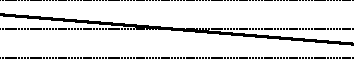
\includegraphics{images/contours-statement.pdf}} //
	\gla Ang gihayo {} Pintemis minganeri-hen yona.//
	\glb Ang giha-yo Ø Pintemis mingan-eri=hen yona //
	\glc \AgtT{} blow-\TsgN{} \Top{} {North Wind} ability-\Ins{}=all
		\TsgN{}.\Gen{}. //
	\glft `The North Wind blew with all of his might.' //
\endgl\xe

\subsubsection{Yes–no questions}

\index{questions!closed}
Since Ayeri does not use a particle or word order to mark closed questions as 
such, intonation is used to mark the difference from a declarative statement. 
To achieve a strong contrast, questions exhibit gradually rising intonation:

\ex[belowexskip=0em]\begingl
	\glpreamble \raisebox{-1.5em}
		{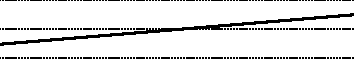
\includegraphics{images/contours-ynquestion.pdf}} //
	\gla Ang gihayo {} Pintemis minganeri-hen yona? //
	\glb Ang giha-yo Ø Pintemis mingan-eri=hen yona //
	\glc \AgtT{} blow-\TsgN{} \Top{} {North Wind} ability-\Ins{}=all
		\TsgN{}.\Gen{}. //
	\glft `Did the North Wind blow with all of his might?' //
\endgl\xe

\subsubsection{`Wh-' questions}

\index{questions!open}
Unlike English, Ayeri marks open questions with an in-situ question word.
Open questions are thus marked by the question word causing a sharp rise and 
fall in the overall contour of the question. The first half of the clause has 
the rising contour of a question, the second half has gradually falling pitch.

\ex[belowexskip=0em]\begingl
	\glpreamble \raisebox{-1.5em}
		{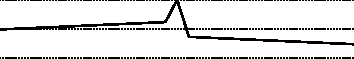
\includegraphics{images/contours-whquestion.pdf}} //
	\gla Ang engyo mico sinya luga toya sam? //
	\glb Ang eng-yo mico sinya-Ø luga toya sam //
	\glc \AgtT{} be.more-\TsgN{} strong who-\Top{} among \TplN{}.\Loc{}
		two //
	\glft `Who was the stronger of the two?' //
\endgl\xe

\subsubsection{Lists}

List statements have the general gradual downward slope of 
declarative statements, but the individual items can nonetheless be marked by a 
pitch rise on the primary accent of each item.

\ex[belowexskip=0em]\begingl
	\glpreamble \raisebox{-1.5em}
		{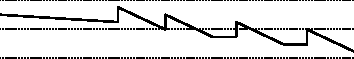
\includegraphics{images/contours-list.pdf}} //
	\gla Le vacyeng seygo, disu, betay nay vasra. //
	\glb Le vac=yeng seygo-Ø, disu-Ø, betay-Ø nay vasra-Ø //
	\glc \PatTI{} like=\TsgF{}.\Aarg{} apple-\Top{}, banana-Ø, berry-Ø and
		nut-Ø //
	\glft `She likes apples, bananas, berries and nuts.' //
\endgl\xe

\subsubsection{Complement and relative clauses}

Complement clauses\index{complement clause} are characterized by the short 
spike at the end of the preceding main clause followed by a short break which 
together signal the beginning of a new syntactic unit within the context of 
the current sentence, which is broadly similar to list statements. Otherwise, 
statements with complement clauses as well bear the overall downward-sloping 
contour of declarative statements if included in such.

\ex\begingl
	\glpreamble \raisebox{-1.5em}
		{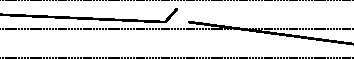
\includegraphics{images/contours-complement.pdf}} //
	\gla Ang manga rantong, engyo mico sinyāng. //
	\glb Ang manga ran=tong, eng-yo mico sinya-ang //
	\glc \AgtT{} \Prog{} argue=\TplN{}.\Aarg{}, be.more-\TsgN{} strong
		who-\Aarg{}//
	\glft `They were arguing who is stronger.' //
\endgl\xe

Relative clauses,\index{relative clause} on the other hand, do not receive 
special prosodic marking, but are treated the same as other basic sentence 
types. They display a continuous downward slope if part of a 
declarative statement, or a continuous upward slope if part of a question:

\pex[belowexskip=0em]
\a\begingl
	\glpreamble \raisebox{-1.5em}
		{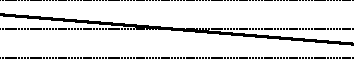
\includegraphics{images/contours-statement.pdf}} //
	\gla Lugaya asāyāng si sitang-naykonyāng kong tovaya. //
	\glb Luga-ya asāya-ang si sitang=naykon=yāng kong tova-ya mato //
	\glc pass-\TsgM{} traveler-\Aarg{} \Rel{} self=wrap=\TsgM{}.\Aarg{} 
		inside cloak-\Loc{} //
	\glft `A traveler passed who had wrapped himself into a cloak.' //
\endgl
\\

\a\label{ex:travelercoat}\begingl
	\glpreamble \raisebox{-1.5em}
		{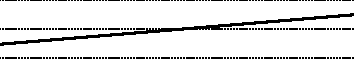
\includegraphics{images/contours-ynquestion.pdf}} //
	\gla Adareng asāyās si le ninyāng tova? //
	\glb Ada-reng asāya-as si le nin=yāng tova-Ø //
	\glc that-\AargI{} traveler-\Parg{} \Rel{} \PatTI{} wear=\TsgM{}.\Aarg{} 
		coat-\Top{} //
	\glft `Is that the traveler who wore the coat?' //
\endgl
\xe

\subsubsection{Contrast}

Ayeri uses a kind of topic system\index{topic} for highlighting constituents in 
a clause by morphosyntactic means, but this is still different from emphasis on 
semantic grounds, for example when the speaker wants to highlight a 
semantic difference in the same syntactic position, as in the following example, 
which presents a possible answer to the question posed in 
(\ref{ex:travelercoat}):

\ex\begingl
	\glpreamble \raisebox{-1.5em}
		{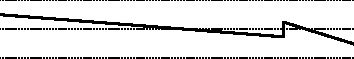
\includegraphics{images/contours-contrast.pdf}} //
	\gla Adareng asāyās si le nin-yāng \upshape{kegan}. //
	\glb Ada-reng asāya-as si le nin=yāng kegan-Ø //
	\glc that-\AargI{} traveler-\Parg{} \Rel{} \PatTI{} wear=\TsgM{}.\Aarg{} 
		hat-\Top{} //
	\glft `It is the traveler who wore the \emph{hat}.' //
\endgl\xe

We can see here a spike towards the end of the utterance where the word 
\xayr{kegnF}{kegan}{hat} is placed. This word receives extra stress for 
contrast with \xayr{tov}{tova}{coat}, which is what the other person had asked 
about.
